\documentclass{seuthesis}

\usepackage{float}        % 支持 [H]（如果仍需要）
\usepackage{placeins}     % 防止浮动体乱窜
\usepackage{enumitem}
\usepackage{xcolor}
\usepackage{listings}
\setlist[enumerate,1]{label=(\arabic*)}

% 定制 Java 代码样式
\lstset{
	language=Java,
	basicstyle=\ttfamily\small,
	keywordstyle=\color{blue},
	commentstyle=\color{gray},
	stringstyle=\color{red},
	numbers=left,
	numberstyle=\tiny\color{gray},
	stepnumber=1,
	numbersep=5pt,
	backgroundcolor=\color{gray!5},
	frame=single,
	rulecolor=\color{black!30},
	breaklines=true,
	breakatwhitespace=true,
	showspaces=false,
	showstringspaces=false,
	showtabs=false,
	tabsize=2,
	captionpos=b           % 标题在下方
}

\newcommand{\demobox}[2]{\fbox{\rule{0pt}{#2}\rule{#1}{0pt}}}

\addkey{机器学习}{ML}
\addkey{关键词 2}{Keyword2}
\addkey{关键词 3}{Keyword3}
\addkey{关键词 4}{Keyword4}

\seusetup{
  title                          = {面向企业级场景的汽车},
  subtitle                       = {数字化运营平台的升级开发},
  author                         = {高晨荐},
  student_id                     = {71122234},
  school                         = {软件学院},
  major                          = {软件工程},
  supervisor                     = {廖力},
  date_range                     = {2026.01.06——2026.06.26},
  cover_date                     = {2026-04-10},
  originality_date               = {2026-04-10},
  authorization_author_date      = {2026-04-10},
  authorization_supervisor_date  = {2026-04-10},
  ai_scope                       = {2},
  ai_used                        = yes,
  ai_checkbox_style              = checkedbox,
  signature_student_image        = {imgs/zhangsan.png},
  signature_teacher_image        = {imgs/zhangsanfeng.png},
  ai_student_date                = {2026-04-10},
  ai_teacher_date                = {2026-04-10},
  ai_teacher_comment             = {同意。}
}

\seuaiitem{
  tool_version = {DeepSeek-V3.2\par ChatGPT-5.4\par Gemini-3.1\par Claude-4.6},
  process = {输入章节主题、关键术语和改写要求，辅助生成初稿表述并对部分段落进行语言润色，最终内容均由本人核对修改。},
  pages   = {第二章 1.1（P5）、第二章 1.2（P7）}
}

\begin{document}

% 封面、独创性声明等（查重不需要，注释掉）
\seumakefrontmatter
% 无实际内容输出，仅做页面格式切换（注释掉）
\seuprefacematter
% 摘要标题 + 关键词——保留
\seumakechineseabstract
% Abstract 标题 + Keywords——保留
\seumakeenglishabstract
% 目录——保留
\seumaketableofcontents
% 正文开始——保留
\seumainmatter
\chapter{绪论}

\section{研究背景和意义}

随着全球汽车工业加速迈向数字化与智能化，“软件定义汽车”（SDV）这个理念已逐步成为下一阶段汽车产业的演进方向。在这一趋势下，车辆的创新焦点和核心价值逐步由传统的机械底盘与动力系统，转移至底层的中央计算平台与上层的高阶软件架构。软件不仅能够影响智能座舱的交互体验与智能驾驶的安全边界，更赋予了车辆在全生命周期内通过无线（OTA）技术持续进化、按需解锁新功能的能力\cite{ibmsoftwaredefinedvehicle}。然而，这种软件规模与复杂度的爆炸式增长，也给汽车电子研发带来了前所未有的质量治理挑战。车规级软件作为关乎人身财产安全的强安全关键系统，对安全性、可靠性有着比较苛刻的行业壁垒与法规要求，必须严格遵循ISO26262功能安全标准及ASPICE（汽车软件过程改进和能力评估）等行业过程模型\cite{mathworks_aspice}。任何微小的软件缺陷若未能及时拦截，那到了量产阶段，都将面临极其高昂的亏损成本，甚至引发重大安全隐患。因此，构建一套高效、严密的软件项目全生命周期管理与项目质量监控体系，已成为当今汽车电子软件行业的迫切工程需求。

另一方面，在传统信息化建设模式下，企业内部各业务系统通常由不同部门独立建设，系统之间缺乏统一的数据协同机制，容易形成“数据孤岛”现象。这种模式不仅降低了数据共享效率，也增加了企业在运营分析、项目管理以及决策支持等方面的难度。随着企业数字化转型不断推进，企业对于运营效率、项目协同能力以及数据利用水平提出了更高要求，传统分散式的信息管理方式已经难以满足实际业务发展的需要。在此背景下，数字化运营平台逐渐成为企业数字化建设的重要组成部分。通过对企业运营数据、项目数据以及研发流程数据进行统一整合与集中管理，数字化运营平台能够实现数据资源的高效共享与协同利用，为企业运营管理、项目进度跟踪、资源调度以及经营决策提供数据支撑，从而提升企业整体管理效率和运营水平。

通过数字化运营平台的建设，企业能够有效打通不同业务系统之间的数据壁垒，缓解传统模式下数据分散、协同效率低等问题，进一步提升部门之间的信息共享与业务协同能力。同时，平台还能够为企业运营管理、项目监控以及资源配置提供更加及时、准确的数据支持，帮助管理人员更好地掌握项目进展和企业运行状态，提高决策的科学性与管理效率，从而增强企业整体运营能力和市场竞争力。

\section{国内外研究现状}

现代项目管理方法体系的形成与大型工程项目、国防工程和信息系统建设密切相关。随着项目规模不断扩大，传统依靠人工经验进行计划安排和过程控制的管理方式逐渐难以满足复杂项目的管理需求，项目管理开始向科学化、规范化和体系化方向发展。国外项目管理理论较早形成了较为成熟的方法体系，逐步将项目范围、进度、成本、质量、风险、沟通和资源等内容纳入统一管理框架。随着项目管理专业化程度不断提高，项目经理逐渐成为企业组织中的重要管理角色，项目管理办公室也逐步承担起项目规范建设、过程监督、资源协调和决策支持等职能。

20 世纪 90 年代以后，随着计算机技术、网络技术和数据库技术的发展，项目管理软件系统逐渐成熟，并被广泛应用于工程建设、软件研发、企业运营和组织管理等领域。国外较有代表性的项目管理软件包括 Microsoft Project、Jira、Asana等，这些系统通常围绕计划编制、任务分配、进度跟踪、缺陷管理、版本管理和团队协作等功能展开。随着敏捷开发、DevOps 和数字化运营理念的发展，国外项目管理系统逐渐由单一的计划管理工具向协同化、平台化和数据驱动方向演进，越来越重视项目过程数据的采集、分析和可视化展示，以支持管理者进行项目监控和决策分析。

国内项目管理信息化建设起步相对较晚，但伴随企业信息化和互联网行业的发展，项目管理软件系统也得到了较快发展。国内常见的项目管理和研发协作工具包括禅道、阿里巴巴的Aone、 腾讯的TAPD 等，这些系统在任务协作、需求管理、缺陷跟踪、文档管理、版本发布和项目统计等方面提供了较为完整的功能支持。与此同时，企业微信、钉钉、飞书等协同办公平台的普及，也推动了企业管理系统向在线化、协同化和轻量化方向发展。对于企业而言，项目管理系统已经不再只是项目经理记录任务和进度的工具，而是逐渐成为连接组织、人员、项目、流程和数据的重要管理平台。

从系统架构角度看，主流项目管理系统大致可以分为 C/S 架构和 B/S 架构两类。C/S 架构即客户端/服务器架构，通常具有响应速度较快、客户端能力较强和安全性较高等优点，但在客户端安装、版本升级和后期维护方面成本较高。B/S 架构即浏览器/服务器架构，用户通过浏览器即可访问系统，不需要单独安装客户端，具有部署方便、维护成本低、跨平台能力强等特点。随着网络基础设施不断完善以及 Web 前端技术的快速发展，B/S 架构在企业管理系统、项目管理系统和数字化运营平台中的应用越来越广泛，逐渐成为企业内部管理平台建设的主要形式。

从功能设计角度看，当前项目管理系统大致可以分为两类。一类是以研发项目管理为核心的专业化系统，如 Jira、禅道等，这类系统通常围绕产品、需求、项目、测试、缺陷、版本和发布等场景进行设计，功能较为完整，能够满足软件研发团队较复杂的过程管理需求，但由于功能模块较多，业务流程相对细致，用户学习成本和系统配置成本也相对较高。另一类是面向企业通用协作和数字化管理的平台型系统，这类系统通常通过字段配置、流程配置、权限配置、表单配置和数据看板等方式适配不同业务场景，具有较强的灵活性和复用性，适合企业根据自身管理流程进行定制化使用。基于B/S架构，简单易上手的软件项目管理系统必将是未来发展的方向 。

\section{论文的组织结构}

本文共分为七章，各章内容安排如下：

第一章为绪论。首先阐述了课题的研究背景与意义，分析了当前汽车电子软件行业在数字化项目质量管理中面临的核心痛点；继而梳理了国内外在研发效能管理、项目质量度量及相关技术领域的研究现状；最后概述了本文的主要研究内容与论文的整体组织结构。

第二章为相关开发技术与环境。对系统开发过程中涉及的关键技术进行了概述，包括后端的SpringBoot框架、前端的Vue框架及其MVVM架构模式、MySQL与Redis的数据存储与缓存方案、ECharts数据可视化库以及MyBatis-Plus持久层框架，为后续的系统设计与	实现提供技术基础。

第三章为需求分析。从系统总体需求出发，结合普通员工、软件项目经理和部门经理三类核心角色的使用场景，分别对BU工时统计分析、项目信息管理、缺陷管理和重大问题管理四个模块进行了功能性需求分析，并从性能、可靠性与易用性等角度提出了非功能性需求。

第四章为系统总体设计。从宏观层面阐述了系统的前后端分离架构，将系统自上而下划分为前端展示层、请求处理层、业务逻辑层、数据访问层和数据层五个层次，并从业务维度将系统横向解耦为系统管理、公司运营管理和项目运营管理三大核心模块，明确了各模块的职责边界。

第五章为核心业务模块的详细设计。在概要设计的基础上，对BU工时统计分析、项目基本信息管理、缺陷管理和重大问题管理四个核心模块进行了详细设计，结合类图与时序图阐述了各模块的业务逻辑与数据流转过程，并给出了数据库的E-R模型与关键表结构设计。

第六章为系统实现与测试。展示了系统核心功能模块的实现效果，并通过功能性测试验证了各业务模块的逻辑正确性，同时从边界测试、安全性测试和性能测试三个维度对系统的非功能性指标进行了评估。

第七章为总结与展望。对本文的研究工作和主要成果进行了总结，分析了系统当前存在的不足，并对后续的改进方向与功能扩展进行了展望。

\chapter{相关开发技术与环境}
\section{SpringBoot框架}
\subsection{SpringBoot框架核心理念}
在Java企业级应用的演化进程中，以Spring、Spring MVC及MyBatis为代表的传统架构曾占据主导地位。然而，这类架构在实际工程落地时，往往伴随着繁杂的XML文件配置、冗长的依赖版本管理以及多步骤的部署流程。开发人员在启动新项目时，必须耗费大量精力去处理各类框架间的整合与组件装配，无形中降低了生产效率。为打破这一应用僵局，Spring Boot框架应运而生。

作为Spring生态体系的深度扩展，Spring Boot的设计初衷是实现“开箱即用”。其最核心的指导原则在于“约定优于配置”。该机制通过提供科学的默认参数，极大地削减了传统开发模式下的样板代码与配置文件。在日常开发中，无需进行繁琐的底层结构搭建，仅需通过少量的注解指令即可接管Bean的管理与自动化装配。这种轻量化的框架重构，不仅使得Web应用的搭建更加灵活，也让开发者的精力得以从底层环境部署中抽离，重新聚焦于核心业务逻辑的实现。
\subsection{SpringBoot框架关键特性}
在现代软件工程中，Spring Boot之所以能够逐渐取代老旧的开发模式，主要得益于其独具优势的几大核心技术特性：
\begin{enumerate}[label=(\arabic*)]
	\item \textbf{解耦机制：}
	继承自Spring生态的底层精髓，Spring Boot深度践行了控制反转（IoC）理念。对象组件的创建与生命周期管理不再由开发者在代码中硬性实例化，而是全权交由框架的IoC容器统一调配。借助依赖注入（DI）技术，系统在运行期间能够通过简单的注解，将关联的实例动态注入到目标对象中。这种机制从根本上剥离了业务模块间的强耦合关系，极大地提升了系统的可测试性与扩展性。
	\item \textbf{起步依赖：}
	框架提供了一种高度聚合的构建与依赖管理方案。结合Maven等项目构建工具，Spring Boot将特定功能场景（如Web通信、安全框架等）所需的庞杂底层类库，封装为标准化的“起步依赖”。当开发者在项目的pom.xml文件中引入某一Starter时，其核心依赖管理机制能够自动下载所需库文件并处理传递性依赖，彻底解决了以往手动排查Jar包冲突的繁琐问题，显著提升开发效率。
	\item \textbf{外部化配置：}
	在企业级软件生命周期的演进过程中，系统往往需要经历本地开发、集成测试与正式生产等多个阶段。面对不同环境下各异的数据库网关、中间件端口及第三方服务密钥等差异化参数，Spring Boot 提供了极具弹性的外部化配置机制。开发团队可以为特定的运行环境预设独立的分支配置文件（如 application-dev.yml 与 application-prod.yml）。在项目构建打包后，运维人员无需对系统源码进行任何重新编译或修改，仅需在服务启动时通过命令行参数、系统环境变量或注册中心，动态声明当前激活的配置集，即可完成复杂环境的无缝切换。这种设计模式，彻底实现了核心业务代码与物理环境参数的深度解耦，极大地提升了项目的交付效率与工程化管理水平。
	\item \textbf{内嵌式运行容器：}
	传统Java Web项目通常需要打包为War格式，并强依赖于外部配置好的Tomcat服务器进行部署。Spring Boot则打破了这一常规，其内部直接集成了主流的Web容器环境。通过打包指令，整个项目及其运行环境可被封装为一个独立的可执行Jar包。只需极简单的终端命令行交互即可直接启动服务，这不仅简化了运维层面的操作步骤，更使其成为现代微服务架构体系下的首选基础框架。
	% 表格与下文之间空一行
\end{enumerate}

\section{Vue框架}
在现代前端工程化实践中，Vue.js 凭借其轻量级与“渐进式”（Progressive）的设计理念，已成为构建交互式用户界面的主流方案之一。所谓渐进式，即该框架允许开发者根据项目复杂度，从简单的页面局部视图增强，平滑过渡到基于全家桶构建复杂的单页应用（SPA）。与传统强依赖频繁操作真实 DOM 节点的库（如 jQuery）不同，Vue2 框架在底层深度贯彻了 MVVM（Model-View-ViewModel）架构模式，如图\ref{fig:mvvm-pattern-diagram}所示。
\begin{figure}[htbp]
	\centering
	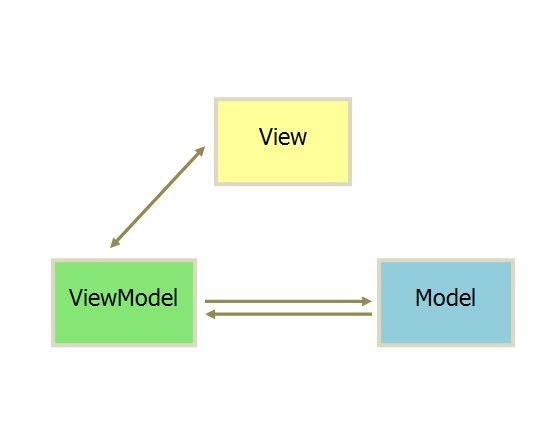
\includegraphics[width=0.68\linewidth]{imgs/MVVM模式图.jpg}
	\caption{MVVM模式图}
	\label{fig:mvvm-pattern-diagram}
\end{figure}

在该架构中，Model 层负责业务逻辑与数据状态的存储；View 层代表视觉呈现界面；而 ViewModel 层则是 Vue 框架的核心枢纽。ViewModel 通过数据绑定技术将数据模型与视图结构桥接起来，当模型数据发生变更时，视图会自动进行同步更新；反之，当用户与视图产生交互时，数据的状态也会被即时捕获。这种双向通信机制彻底剥离了繁琐的底层节点操作，使得前端工程的重心得以回归到核心业务数据的流转上。

主流的前端框架除了Vue，还有React和Angular。对比于 React 框架，Vue 在视图渲染效能、语法直观性及周边生态储备上表现出显著的优越性。在页面重绘机制上，Vue 依托精细的响应式追踪机制配合虚拟 DOM 与 Diff 算法，能够以极高的精度定位视图层中需变更的最小范围，从而大幅削减不必要的渲染开销。就编码体验而言，其高度提炼的模板语法极大地降低了代码的晦涩感，提升了业务模块的开发速率。同时，其背后沉淀的庞大开源社区与海量高质量插件，为复杂功能的快速落地提供了坚实的扩展支撑。
另一方面，相较于体量庞大的 Angular ，Vue 有着轻量化的架构设计、平缓的学习曲线以及高内聚的模块化管理。它摒弃了冗余的默认规范约束，赋予了项目极高的配置自由度，使工程脚手架的搭建能够精准贴合实际业务诉求。其出色的架构弹性不仅允许作为独立库无缝嵌入传统项目，还能在组件化模式下保持数据流转的清晰透明，极大便利了后期的代码审阅与缺陷排查。

结合本系统对开发周期、代码可维护性以及复杂表单交互效率的工程要求，Vue 框架具备轻量灵活、学习成本低、生态完善等优势，因此选择 Vue 来搭建系统的前端。

\section{数据库技术}
在企业级 Web 应用的系统架构中，数据持久化与高并发读写性能是衡量系统健壮性的核心指标。为了兼顾数据的强一致性约束与系统的高频访问响应速度，本系统在数据存储层采用了MySQL来进行数据的持久化，利用Redis的高性能来降低接口响应时间。
\subsection{关系型数据库MySQL}
MySQL 是目前全球应用最为广泛的开源关系型数据库管理系统之一，它的基础架构基于C++实现，因此有着卓越的查询性能。MySQL官网支持主流的操作系统，有着极低的部署成本以及庞大的开发者生态。其运行机制如图\ref{fig:sql-execution-diagram}所示。
\begin{figure}[htbp]
	\centering
	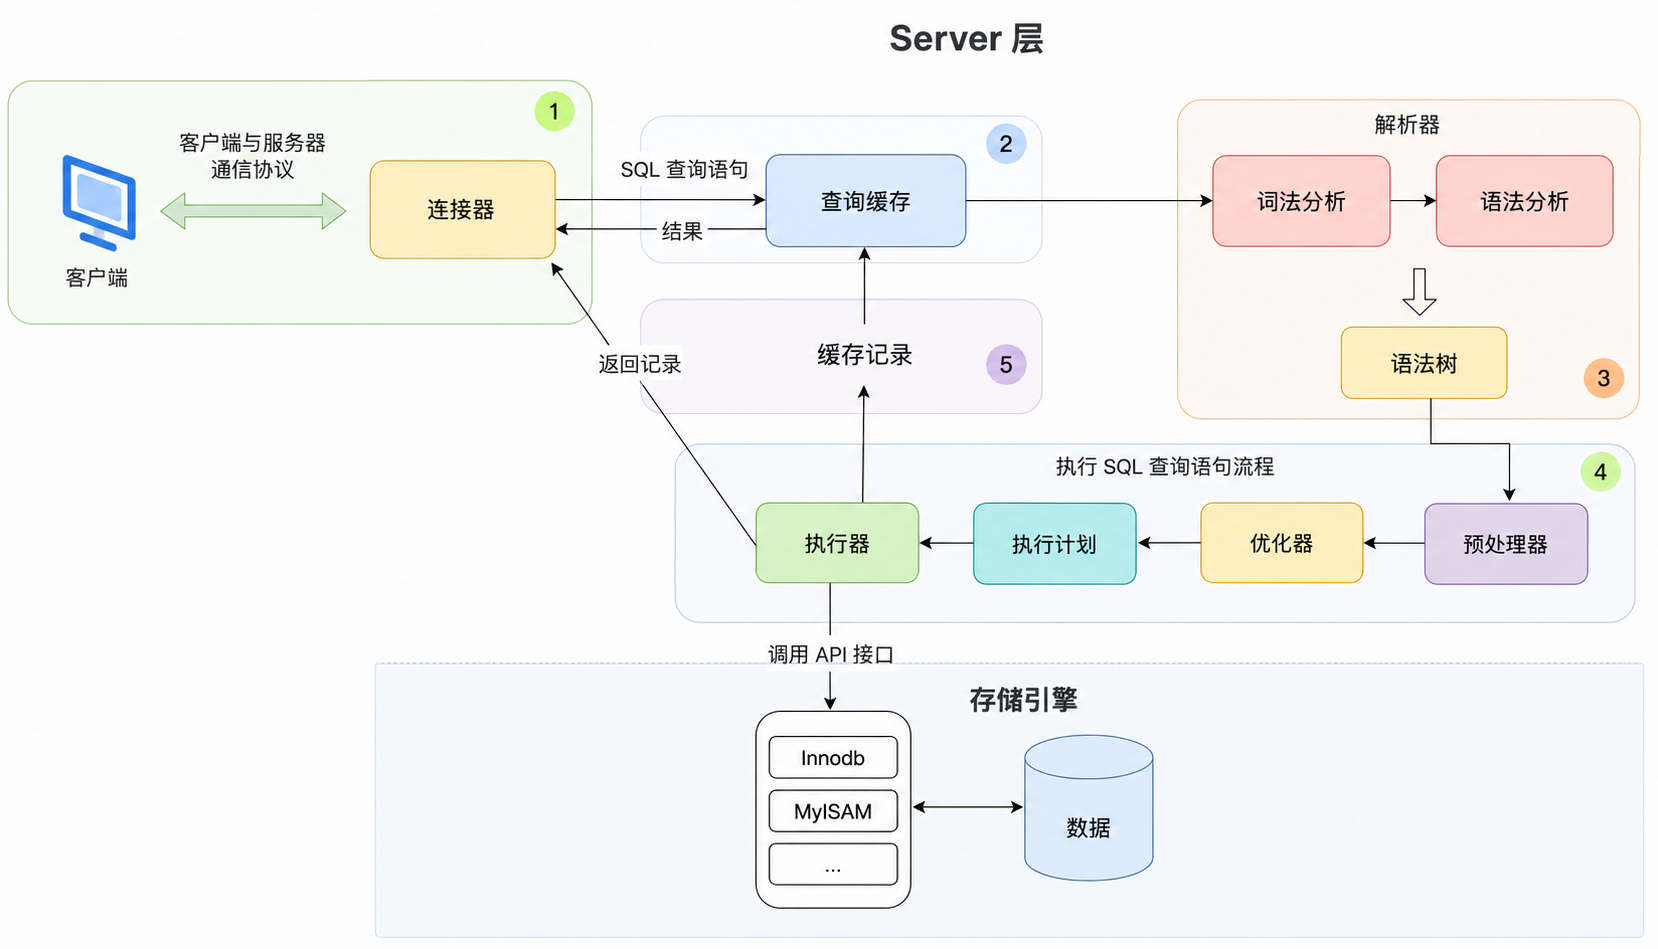
\includegraphics[width=0.68\linewidth]{imgs/SQL执行过程.png}
	\caption{MySQL执行流程图}
	\label{fig:sql-execution-diagram}
\end{figure}

客户端通过TCP协议连上 MySQL 服务后，会先做权限校验和身份确认，这一步由连接器负责，为了提高速度和资源利用率，MySQL会用连接池来进行连接。接着，系统会看看之前有没有执行过一模一样的 SQL（但是查询缓存在最新的MySQL版本中因为命中率太低被移除了）。之后这条查询语句会走到解析器那里，做词法和语法检查，看看语句写得对不对；然后再交给预处理器，验证里面涉及的表和字段是不是真的存在。再往后就是优化器登场，它会根据各种情况算一算哪种执行方案成本最低，比如决定用哪个索引来查。最后执行器按这个计划去调用存储引擎提供的接口，把符合条件的记录一条条取出来，最终将结果集打包返回给客户端。

本系统选用其默认的 InnoDB 存储引擎，该引擎不仅提供了对 ACID（原子性、一致性、隔离性、持久性）事务的完整支持，底层更依托 B+ 树数据结构构建索引，极大地优化了数据检索的磁盘 I/O 效率。同时，InnoDB 通过引入 MVCC（多版本并发控制）机制与行级锁，有效解决了高并发场景下的读写冲突，保障了多线程环境下的数据隔离与一致性。
\subsection{非关系型数据库Redis}
虽然 MySQL 能够提供稳定可靠的数据持久化服务，但在面对海量并发访问或热点数据高频查询等低延迟交互场景时，传统关系型数据库易面临严重的磁盘 I/O 瓶颈，为此，本系统引入了 Redis 作为非关系型数据库。Redis 本质上是一款由c语言实现的，基于内存的高性能键值对存储系统，由于其数据读写操作主要在 RAM 中进行，能够实现亚毫秒级的响应延迟与极高的吞吐量。除了基础的字符串类型，Redis 还原生支持哈希、列表、集合、有序集合等丰富的数据类型，开发者能够很便捷地将其应用于排行榜，分布式锁，打卡签到等场景。为了兼顾数据安全性，Redis提供了RDB快照和AOF日志两种持久化方式，前者定期保存全量数据，后者以追加形式记录每条写命令，两者可组合使用或采用混合持久化以平衡恢复速度与数据完整性。在性能方面，Redis采用单线程模型处理命令，避免了多线程的锁竞争和上下文切换开销，同时借助I/O多路复用技术让单个主线程能够并发处理大量客户端连接。基于以上特性，在流量较大或者数据库查询比较慢的接口，引入 Redis 可以有效减少到达数据库的请求数量，提高系统的性能和稳定性。

\section{Echarts库}
ECharts是一款基于JavaScript编程语言实现的开源Web数据可视化库，常用于在网页中呈现各类统计图表。该库支持折线图、柱状图、饼图、散点图以及地图等多种常见图表类型，并且允许在同一图表中组合多种图形。开发时只需通过一个配置对象指定图表的样式与数据，ECharts便会自动完成渲染，并内置了缩放、悬停提示等交互功能。底层可选用Canvas或SVG两种渲染方式，能够适应从少量数据到大规模数据的展示需求。在本系统的前端模块中，使用ECharts将后台统计数据以直观的图表形式呈现，便于用户快速获取信息。

\section{MyBatis-Plus}
MyBatis-Plus是一个基于Java编程语言实现的持久层框架，它在MyBatis的基础上提供了一层轻量级的封装，核心设计理念是“只做增强不做改变”，即完全兼容原生MyBatis的所有特性，同时通过内置通用Mapper、条件构造器和代码生成器等组件大幅简化数据库访问层的开发工作。在实际使用中，持久层接口只需继承MyBatis-Plus提供的BaseMapper接口，即可自动获得单表增删改查的全部方法，无需为每个表手动编写相应的SQL语句和映射配置。对于查询条件较为复杂的场景，MyBatis-Plus提供了灵活的Wrapper条件构造器，支持通过Lambda表达式以编程方式动态拼接WHERE条件，不仅规避了XML配置文件中SQL语句的编写工作，还通过方法引用的形式避免了字段名拼写错误等潜在问题。在批量数据处理和分页查询方面，该框架内置了分页插件，能够在数据库层面实现物理分页，开发者只需传入页码和每页条数即可完成分页查询，无需关心底层不同数据库的分页语法差异。对于多表关联查询等复杂场景，MyBatis-Plus保留了手写SQL的能力，开发者仍可在XML或注解中编写原生MyBatis语句，与框架提供的通用CRUD操作共存互补，兼顾了开发效率与底层控制的灵活性，使得开发者能够将更多精力聚焦于业务逻辑，在Java后端项目中被广泛采用。

\section{本章小结}
本章围绕系统开发所依赖的关键技术进行了概述。后端采用SpringBoot框架，借助其自动装配与内嵌容器机制简化服务端开发与部署流程；前端选用Vue框架，介绍了MVVM模式实现视图与数据的双向绑定，降低前端交互的开发复杂度。数据层采用MySQL与Redis组合方案，前者用来管理系统持久化到磁盘的数据，后者通过内存缓存加快响应速度。MyBatis-Plus简化了持久层的CRUD编码，ECharts为数据可视化提供了图表支撑。
\chapter{需求分析}
需求分析是软件工程生命周期中十分关键的环节，其主要任务是通过对用户需求、业务场景和实际问题的梳理，将较为抽象的业务想法转化为清晰、可执行、可验证的需求说明。需求分析的质量直接影响系统建设的范围、设计方向以及最终交付效果，是连接业务目标与技术实现的重要基础。

本章围绕企业数字化运营平台的建设需求展开分析。首先，对系统应具备的总体功能进行概述，使读者能够从整体上了解系统建设的背景和意义；随后，进一步从功能需求和非功能性需求两个方面进行分析。其中，功能需求主要描述系统各业务模块应实现的具体功能，是后续系统架构设计、模块划分和业务流程设计的重要依据。非功能性需求则主要关注系统在实际运行过程中的稳定性、安全性、可扩展性和易用性等方面，既要保证系统能够长期稳定运行，也要提升用户在使用过程中的流畅性、便捷性和可靠性。

\section{系统总体需求概述}
本系统是某汽车电子公司内部的数字化运营管理系统，面向企业内部的软件项目管理和运营管理场景，主要用于解决项目过程数据分散、统计分析依赖人工整理、业务流程跟踪不能自动化等问题。系统需要将项目、组织、人员、工时、质量和运营指标等数据进行整合，为管理人员提供较为统一的数据查看和业务处理平台。

从业务范围上看，系统主要包括三个部分。第一部分是项目管理，围绕项目基础信息、版本范围、质量问题和风险事项等内容，对项目执行过程进行记录、查询和跟踪。第二部分是公司运营管理，主要面向组织、员工、工时和 KPI 等运营数据，支持从部门、人员、项目等角度进行统计分析。第三部分是系统管理，该部分主要作为系统基础支撑，提供用户、角色、菜单、部门、权限和日志等后台管理功能，为业务模块的正常运行提供支撑。
\begin{figure}[htbp]
	\centering
	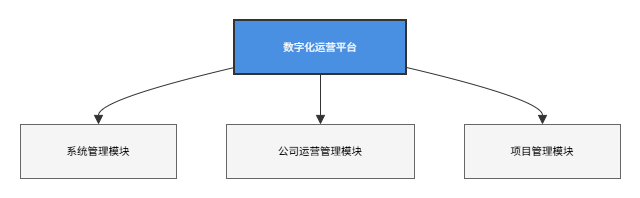
\includegraphics[width=0.68\linewidth]{imgs/总体模块图.png}
	\caption{玄武平台模块图}
	\label{fig:xuanwu-module}
\end{figure}

系统的使用对象包括项目经理、部门经理、项目成员（开发测试人员）以及质量管理人员等。不同角色在系统中的关注内容和操作权限不同，因此系统需要具备统一的身份认证、权限控制和数据访问管理能力，以保证业务数据的安全性。本系统的建设目标是将项目管理、运营分析和系统基础管理整合到同一平台中，减少分散系统和人工统计带来的管理成本，提高企业内部项目过程管理和运营数据分析的效率。

\section{功能需求}
在系统总体需求的基础上，本节结合毕业设计任务分工，对本文负责实现的功能模块进行需求分析。本文的实现范围主要包括公司运营管理模块中的部门投入 BU 工时统计功能，以及项目管理模块中的项目基础信息管理、缺陷管理和重大问题管理功能。上述功能分别对应运营数据分析和项目过程管理两个方面，是系统整体业务中的一部分。

在相关功能中，部门经理主要关注部门工时在不同 BU 方向上的投入情况；项目经理主要负责项目基础信息维护和项目过程跟踪；项目成员（开发测试人员）参与缺陷和重大问题的处理与反馈；质量管理人员则重点关注缺陷数据、重大问题状态以及相关质量风险。为便于后续系统设计，下面将按照功能模块分别分析各功能的参与角色、业务目标和主要操作需求。

\subsection{部门投入BU工时统计需求分析}
BU工时投入分析模块旨在为部门经理提供下属员工在各BU（Business Unit）上工时分布的全景视图，为人力资源调配与项目成本核算提供数据支撑。该模块仅涉及部门经理一类参与者。如图\ref{fig:bu-usecase}所示，系统需要提供按年月和组织树两个维度的工时数据检索能力，支持以饼图形式呈现部门整体的BU工时分布情况。同时，系统需要支持对特定BU的工时数据进行详细分析，提供总工时、平均工时和加班工时等基础统计指标的计算能力，并能够生成近六个月的工时趋势图，以便识别工时投入的变化规律。
\begin{figure}[htbp]
	\centering
	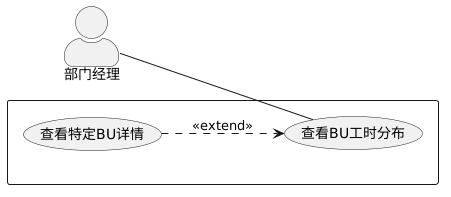
\includegraphics[width=0.68\linewidth]{imgs/usecase/部门投⼊到BU的⼯时分布用例图.png}
	\caption{BU工时分布用例图}
	\label{fig:bu-usecase}
\end{figure}

\subsection{项目信息管理需求分析}
项目信息管理模块需要支持项目经理、项目成员这两类参与者对项目基本信息和里程碑计划的。如图\ref{fig:project-usecase}所示，该模块可划分为项目基本信息和里程碑计划两个子域。在项目基本信息方面，系统需要支持项目信息的新增、编辑、查询和导出能力，其中项目经理拥有完整的写权限，部门经理和普通用户仅具备只读权限。在里程碑计划方面，系统需要支持项目周报的填写、修改和查询，以及交付历史的查看，确保各角色能够在各自权限范围内获取所需的项目进度信息。
\begin{figure}[htbp]
	\centering
	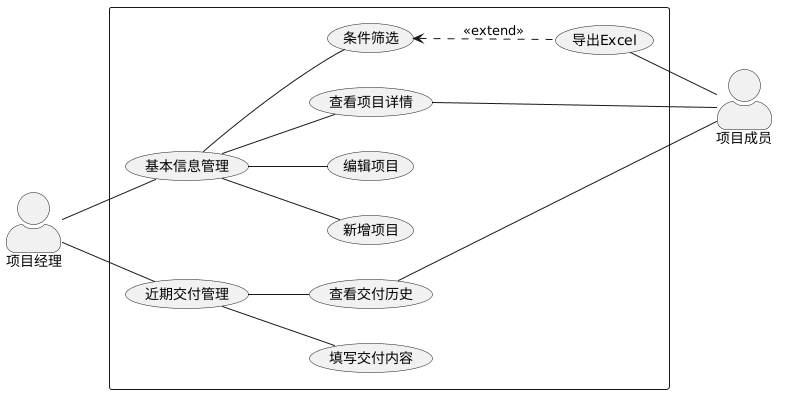
\includegraphics[width=0.68\linewidth]{imgs/usecase/项目信息管理用例图.png}
	\caption{项目信息管理用例图}
	\label{fig:project-usecase}
\end{figure}


\subsection{缺陷管理需求分析}
缺陷管理模块需要解决企业内部缺陷数据分散在多个异构平台中的问题，实现缺陷信息的统一归集与聚类分析。如图\ref{fig:defect-usecase}所示，该模块的用例可归纳为缺陷查看与项目聚类管理两大部分。在缺陷查看方面，系统需要对接Trinity、Jira和BugClose三个外部缺陷跟踪平台，将分散的缺陷数据统一汇总，并支持按项目、集群、时间等多维度进行条件筛选和详情查看，三类角色均可使用该能力。在项目聚类管理方面，系统需要支持项目聚类的增删改查操作，并提供聚类下项目列表和缺陷详单的查看能力；当缺陷数量达到预警阈值时，系统需要具备通过飞书向相关人员发送预警消息的能力。此外，系统还需要支持缺陷数据的Excel导出，便于线下分析和汇报。
\begin{figure}[htbp]
	\centering
	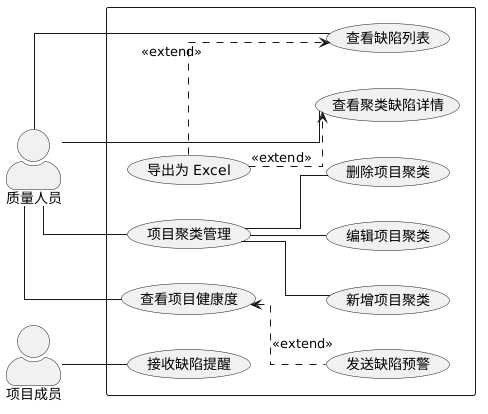
\includegraphics[width=0.68\linewidth]{imgs/usecase/缺陷管理用例图.png}
	\caption{缺陷管理用例图}
	\label{fig:defect-usecase}
\end{figure}

\subsection{重大问题管理需求分析}
重大问题管理模块需要对项目中出现的高影响风险问题提供从登记、跟踪到闭环处置的全流程管理能力。如图\ref{fig:critical-usecase}所示，系统需要支持重大问题的新建、编辑、查询和导出功能，其中编辑功能需要涵盖根因分析、关闭信息填写和问题上升标记三种处置动作。在通知机制方面，系统需要在问题新建或上升时具备通过飞书卡片消息向管理层推送通知的能力。在监督层面，系统需要支持重大问题列表查看、统计图表展示和数据导出，并支持在需要时主动触发飞书催办。此外，当重大问题需要横向扩散时，系统需要支持在问题关闭阶段将横展信息同步推送到其他可能存在相同风险的项目中，确保问题不被遗漏。该模块涉及部门经理、项目经理和普通用户三类参与者，如图\ref{fig:critical-usecase}所示。
\begin{figure}[htbp]
	\centering
	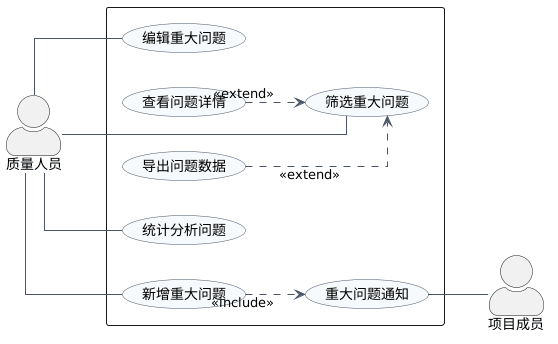
\includegraphics[width=0.68\linewidth]{imgs/usecase/重大问题用例图.png}
	\caption{重大问题用例图}
	\label{fig:critical-usecase}
\end{figure}

\section{非功能需求}
前文主要对系统的核心业务用例和功能流转进行了梳理。但在实际的企业生产环境中，除了要满足基础的业务逻辑外，系统还必须具备在长周期运营与高频使用中的可用性与可靠性，因此，在实际编码之前，本平台还需要满足以下几个关键的非功能性指标。

\subsection{性能要求}
按照汽车软件研发团队的规模推算，系统上线后，底层的工时流水记录和历史缺陷明细表的数据量会在短时间内快速增长，导致单张数据表的体积非常大。这就要求系统在处理涉及多表关联和分组聚合统计时，不能出现严重的慢查询。特别是对于前端首页通过 ECharts 渲染的 BU 工时看板和项目健康度图表，规定相关数据接口的响应时间必须控制在用户可接受的范围以内。如果因为底层数据量过大导致页面出现长达几秒的“白屏”，或者直接抛出请求超时异常，是实际业务无法接受的，因为这非常影响用户的体验。

\subsection{外部接口的容错性}
由于该项目的后端设有定时任务，需要定时调用外部的飞书 API 来向满足条件的用户发送飞书卡片进行催办。但在真实网络环境下，第三方接口随时都可能出现限流、网络波动或定时任务运行出错。因此，系统设计时必须考虑相应的容错处理。具体来说，当调用飞书接口超时或失败时，当前任务线程不能直接崩溃，同时，涉及业务变更的数据库操作必须触发事务回滚，防止产生脏数据。此外，系统需要把这类外部调用异常的堆栈信息完整地输出到日志文件中，并在连续失败时主动向管理员发送告警，以便人工介入排查。

\subsection{接口的健壮性}
Web 应用开发的一个基本原则是“永远不要相信前端传来的数据”。为了防止非法参数引发后台的空指针异常或越权漏洞，所有 Controller 层的入口都必须接入严格的参数校验逻辑，把无效请求直接挡在业务代码之外，降低系统不必要的运算消耗。另一方面，考虑到高并发场景，一些恶意查询或者异常前端代码会频繁查询数据库中不存在的数据，就会导致 Redis 缓存永远无法命中，所有的请求都越过缓存这道防线到达底层数据库，极易引发数据库连接池耗尽甚至宕机。因此，需要采取具体的策略来进行防范，比如最简单的操作就是缓存一些空对象，并设置合适的过期时间。

\subsection{易用性}
由于该运营平台的使用者涵盖了从普通外包测试员工到高层 PMO 经理，各自的使用习惯差异很大，这就要求前端界面不能设计得过于繁琐。前端界面需采用现代化的扁平化设计与组件化交互规范，降低操作门槛。特别是在处理含有几十个字段的工时填报表单或缺陷长列表时，必须做好数据的异步加载、分页以及按钮的“防抖”处理（防止用户手抖连续点击提交）。当数据保存成功或后台校验失败时，系统必须通过全局的消息组件给出明确的中文提示，避免给用户造成“点不动”或“系统卡死”的错觉。

\section{本章小结}
本章围绕企业数字化运营平台的建设目标，从总体需求、功能性需求和非功能性需求三个层面，对系统进行了全面梳理与深度分析。首先从普通员工、项目经理、部门经理等核心用户的视角出发，分析出他们各自的需求。在此基础上，将待实现的功能需求按照业务领域重新聚合，同时从性能、容错、安全与易用性等角度提出了系统在高并发、大数据量场景下的非功能约束。下一章将基于此需求规格，通过描述系统的概要设计来阐述系统的整体架构设计。


\chapter{系统总体设计}
本章对数字化运营平台进行总体设计。先分析了系统的整体架构与分层职责；随后对平台功能模块进行划分，明确本文负责实现的核心功能范围，为后续详细设计与系统实现提供依据。

\section{系统整体架构设计}
数字化运营平台面向企业内部多个部门的项目管理人员和运营团队，使用人员分布在研发、测试和管理等多个岗位，日常办公终端环境存在差异。平台在上线后需要根据业务变化持续迭代功能，对版本发布和升级的便捷性有一定要求。为降低客户端安装、升级和版本维护成本，本文延续 B/S 架构进行设计与开发，用户只需通过浏览器即可访问系统，能够降低终端适配和版本管理的复杂度。

为了降低模块之间的耦合度，并提高系统后续维护和扩展的便利性，本文在整体架构设计中采用分层设计思想，将系统划分为前端展示层、请求处理层、业务逻辑层、数据访问层和数据层五个部分\cite{iso42010_2022}。各层之间按照相对明确的调用关系进行协作，上层主要负责展示结果和接收请求，下层则负责业务处理、数据访问和数据持久化。

具体而言，展示层由前端页面组成，负责用户交互、数据展示和请求发送；请求处理层负责对请求进行身份和权限校验；业务逻辑层负责处理项目管理、公司运营管理等核心业务规则；数据访问层负责封装对数据库的访问操作；数据层则用于保存系统运行过程中产生和同步的业务数据。通过这种分层方式，系统的页面展示、业务处理和数据操作能够保持相对独立，有利于提高系统结构的清晰度。系统整体架构如图~\ref{fig:system-architecture} 所示。
\begin{figure}[htbp]
	\centering
	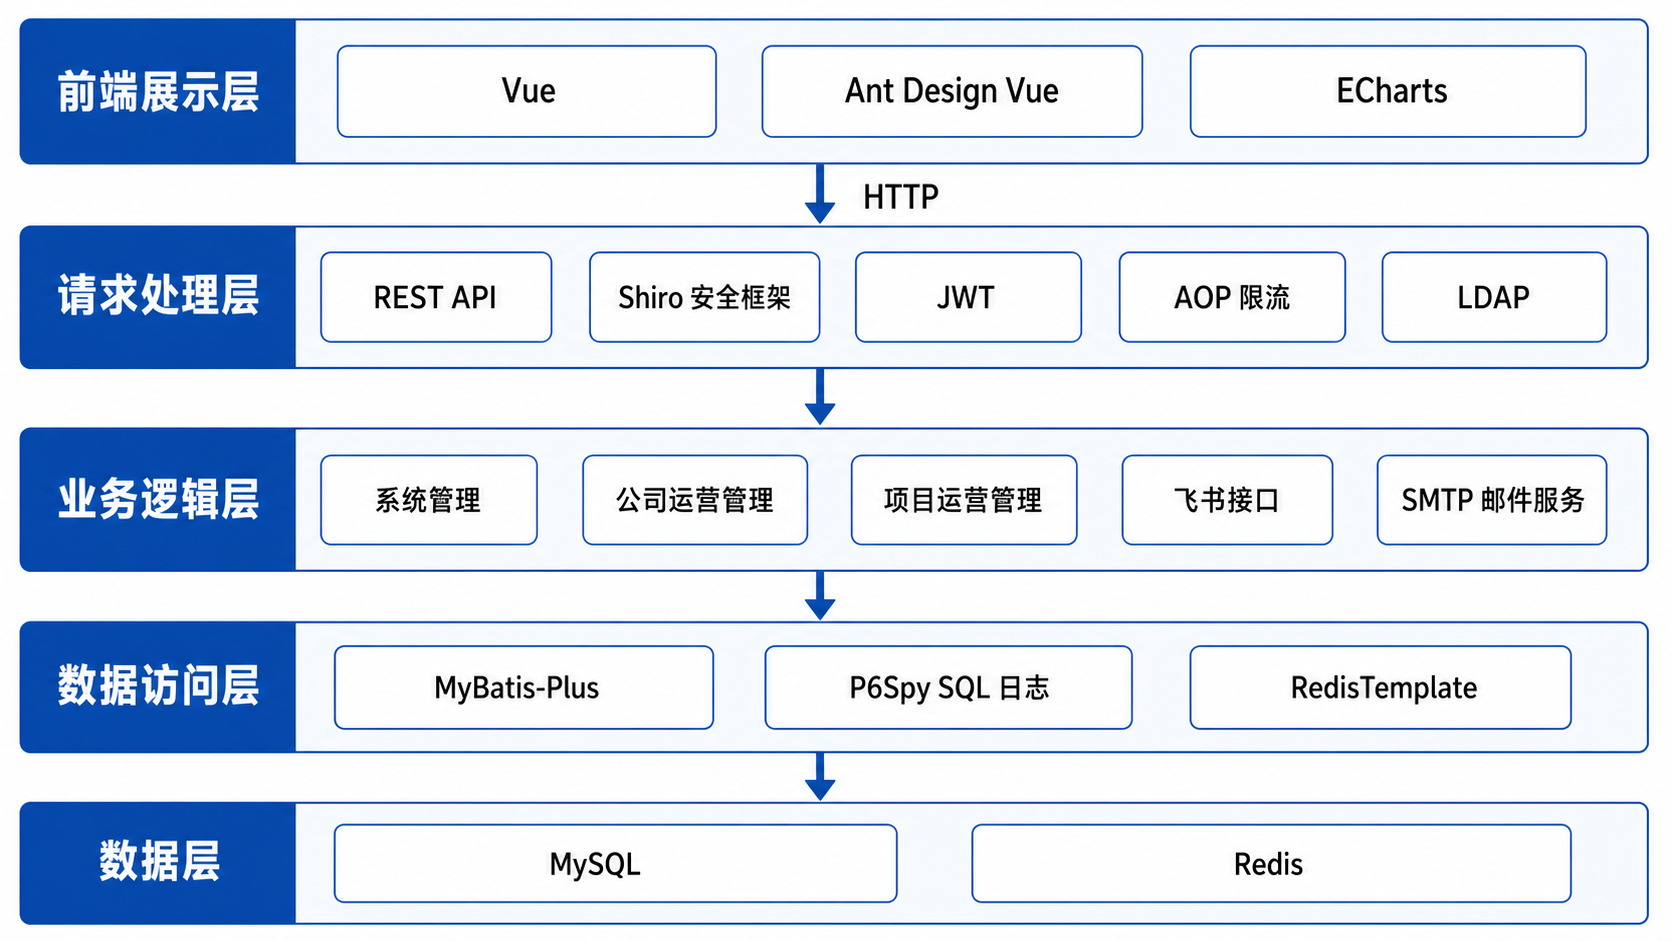
\includegraphics[width=1.0\linewidth]{imgs/arch/系统架构图2.png}
	\caption{系统架构图}
	\label{fig:system-architecture}
\end{figure}

第一层为\textbf{前端展示层}。
负责系统页面展示、用户交互和数据可视化等工作。本系统前端基于 Vue 进行开发，页面组件和基础交互控件主要采用 Ant Design Vue 实现，能够满足表单、表格、按钮、弹窗等后台管理系统常见界面的开发需求。对于数据展示场景，系统使用 ECharts 绘制柱状图、折线图、饼图等可视化图表，使用户能够更直观地理解统计结果。前端通过 Axios 与后端接口进行 HTTP 通信，然后从后端返回的 JSON 格式中拿到数据。前端项目运行环境依赖 Node.js，并通过 npm 管理前端依赖，使用 Webpack 完成项目打包和构建。

第二层为\textbf{请求处理层}。
位于前端界面和后端业务处理之间，主要负责身份认证、权限校验和接口访问控制，作为后端服务的统一“过滤器”。本系统使用 Shiro 安全框架实现用户认证与授权管理，通过 JWT（JSON Web Token）在用户登录后颁发身份令牌，前端在访问登录接口后拿到令牌并保存到本地，后续所有请求都在请求头中携带该令牌，后端对令牌有效性和用户权限进行校验。用户登录时，系统结合 LDAP（Lightweight Directory Access Protocol）进行企业内部的统一身份认证。除身份和权限控制外，系统还通过 AOP 自定义注解方式对部分接口进行限流处理，避免短时间内重复请求对系统造成过大压力。

第三层为\textbf{业务逻辑层}。
该层是系统后端的核心部分，主要负责项目管理、公司运营管理等业务功能的处理。前端发起的 HTTP 请求在通过安全校验后，会根据请求方式和请求路径分发到对应的后端接口，并进入具体的业务模块。
在业务处理过程中，系统首先对请求参数进行必要的校验，保证输入数据符合接口处理要求。对于部分统计类或查询频率较高的数据，业务逻辑层会优先判断缓存中是否存在有效结果；若缓存命中，则直接返回缓存数据，减少重复计算和数据库访问；若缓存中不存在有效数据，则继续执行相应的业务规则处理、数据统计计算和结果封装等操作。业务逻辑层在需要访问数据库时，会调用数据访问层提供的数据访问方法。最终，业务逻辑层将处理结果封装为统一的响应对象，并返回给前端展示。

第四层为\textbf{数据访问层}。
数据访问层负责屏蔽底层数据读写细节。MyBatis-Plus 提供基础的数据访问能力，但是由于过度封装，相比于传统的 XML 手写SQL来说并不是很直观。为了满足查看SQL执行计划的需要，使用P6Spy SQL 日志用于记录和分析 SQL 执行情况，RedisTemplate 用于操作缓存数据。业务逻辑层不直接访问数据库，而是通过这一层提供的接口完成数据查询和写入。

第五层为\textbf{数据层}。
数据层负责系统数据的持久化和缓存支撑。MySQL 存储系统权限、用户、项目、缺陷、运营等核心业务数据；Redis 用于缓存、会话和高频访问数据，提升热点数据查询的响应速度并减轻数据库压力。

\section{系统功能模块划分}
在上述分层架构的基础上，从业务维度对后端工程进行功能模块划分，将系统拆分为三个核心业务域：系统管理、公司运营管理和项目运营管理，以降低模块间的耦合度并提升代码的可维护性。从整体功能上看，项目管理模块主要围绕汽车电子软件过程管理展开，包括项目基础信息、缺陷、重大问题、风险、版本范围等功能；公司运营管理模块主要面向企业组织、员工、工时和KPI等运营数据，支持企业内部运营情况的统计分析；系统管理模块主要包括用户管理、角色管理、菜单管理、系统监控和日志管理等功能，用于保障系统的正常运行。

其中，项目管理和公司运营管理承担主要业务功能，系统管理为业务模块提供用户、权限和菜单等基础支撑。本文根据毕业设计任务分工，重点对其中部分功能模块进行设计与实现，包括公司运营管理下的部门投入 BU 工时分布，项目运营管理下的项目基本信息管理、缺陷管理和重大问题管理，如图\ref{fig:function-module}所示。
\begin{figure}[htbp]
	\centering
	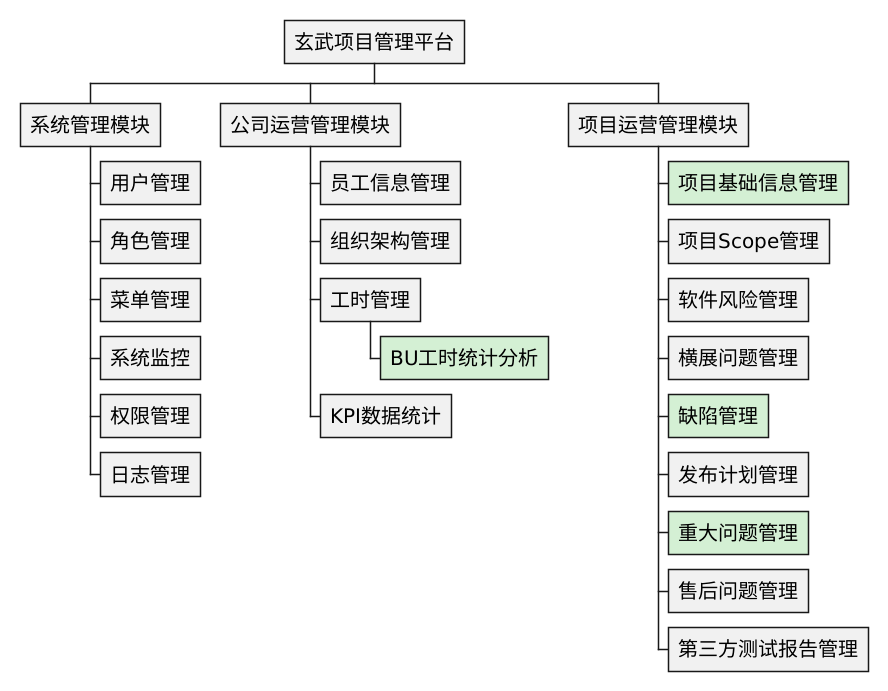
\includegraphics[width=0.7\linewidth]{imgs/玄武功能模块图Detail.png}
	\caption{系统功能模块划分图}
	\label{fig:function-module}
\end{figure}

(1)部门投入BU工时分布

主要用于从部门维度统计各业务单元的工时投入情况。该功能面向管理人员对部门资源投入结构的分析需求，通过对工时数据、员工信息和组织信息进行关联汇总，展示指定部门在不同 BU 方向上的工时分布情况，从而帮助管理人员了解部门人力资源在各业务方向上的投入比例和变化趋势。该功能是部门经理使用的，前端每次发送的请求都会先经过请求处理层看看用户携带的 Token 是否有效，之后会解析出用户的ID,然后通过系统管理模块下的权限校验功能去数据库中查询该用户是否具备权限。
\clearpage

(2)项目基本信息管理

项目基本信息管理主要面向项目经理使用，用于对项目基础数据进行查询和维护，内容包括项目名称、项目类型、所属 BU、里程碑计划、平台、客户以及项目状态等信息。对于项目信息在运行过程中的变更，系统会保留相应的历史记录，从而保证项目数据的可追溯性。该模块也为其他业务功能提供基础数据支撑。例如，在 BU 工时分布中，为满足数据库范式要求，工时数据不会记录项目属于哪个业务单元，还需要关联项目信息表来查询。在新增风险、重大问题时，表单中的下拉框数据也需要使用该模块的接口来查询。

(3)缺陷管理

缺陷管理模块主要用于对项目缺陷数据进行查询、统计和导出，帮助质量人员掌握项目质量状态。这些缺陷数据来自于系统使用的 Trinity、BugClose、Jira 这三个缺陷管理平台，会通过定时任务同步到本地的数据库中。用户可以对缺陷数据进行分页查询，也可以将多个项目看作一个聚类来进行汇总分析。对于健康度较低的项目聚类，质量人员可以发送飞书消息提醒，这里就需要通过组织架构管理和员工信息管理模块的接口来确认消息的接收人员列表。此外，一个缺陷被发现并修复后，可能也会在其他项目中暴露，项目经理可以标记缺陷为需要横展，之后进入横展问题管理模块的流程。

(4)重大问题管理

重大问题管理模块主要用于对项目管理中比较严重的问题进行跟踪和处理。质量人员可以在该模块中维护重大问题的基本信息、责任人、所属项目、客户及处理进展等内容。对于新增或需要重点关注的问题，系统支持通过飞书消息进行通知，使相关责任人能够及时接收到问题信息并开展处理。重大问题可能由风险转入，也可能由横展引发。对一个重大问题，项目经理同样可以标记为需要横展，进入横展的流程。

\section{本章小结}
本章主要对数字化运营平台进行了总体规划与设计。首先从分层角度阐述了系统的五层架构，包含前端展示层、请求处理层、业务逻辑层、数据访问层与数据层，并标注了各层的核心技术栈选型。随后，从实际业务维度出发，将系统拆分为系统管理、公司运营管理和项目运营管理三大核心模块，并简要介绍了本文负责的功能模块主要职责。


\chapter{核心业务模块的详细设计}
上一个章节从整体架构、功能模块等层面对系统进行了宏观设计，明确了各模块的职责。在此基础上，本章将对系统的核心模块展开详细设计，将概要设计转化为可落地代码方案。本章从系统的各个模块和几个关键点设计出发，结合类图与时序图来解释类之间的关系以及核心方法的业务逻辑，为后续的系统实现与测试提供关键性的保障。

\section{系统各模块设计}
这个系统所有模块在工程上都采用了标准的Controller、Service、Mapper三层架构。Controller层定义接口的请求方式、请求路径以及请求参数等，负责接收请求，调用 Service 处理业务逻辑；Service层处理核心业务逻辑和事务，以及调用Mapper或外部服务；Mapper层与数据库进行交互，对于一些复杂的多表操作，由于 Mybatis-plus 只是提供了一些简单的单表操作，因此我们需要在xml文件中编写相应的SQL语句。对于数据查询操作，封装了查询请求基类 QueryRequest ，便于其他模块复用统一的分页（页号，页大小）与排序规则（排序字段、升序开关）属性，各个模块可以根据需求继承该类来扩展特定的业务查询维度。控制层在收到业务层的返回结果后，统一由 FebsResponse 包装后响应给前端。

\subsection{BU工时投入分析}
部门当月投入到各BU（业务单元）的工时分布，是企业管理人力资源调配的重要可视化视图。当前界面默认加载当月的公司整体BU工时饼图，用户可通过年份加月份、组织这两个维度进行筛选。点击某一BU模块后，下方区域将展示该BU的工时详情，包括总工时、平均工时、工时占比、加班工时及工时趋势等关键指标。这些指标数据为项目成本核算与业务决策提供了客观的数据支撑。

如图\ref{fig:class-bu-hour}所示。
\begin{figure}[htbp]
	\centering
	
\includegraphics[width=1.0\linewidth]{imgs/class/BU工时类图.png}
	\caption{BU工时统计类图}
	\label{fig:class-bu-hour}
\end{figure}
在该类图中，WorkHourController通过@RestController标识为 REST 风格的控制器,之后再用@RequestMapping分别定义各个接口的请求方法和路径,接收前端传入的年份、月份、组织节点及 BU 名称等检索条件，为了避免接口参数的散乱以及提高代码的可读性与扩展性，将其统一封装为 WorkHourQueryDTO 数据传输对象。业务层先通过service接口定义规范，模块的核心业务在实现类WorkHourServiceImpl中进行重写，该服务类中通过注解@Autowired注入了多个持久层对象：包括用于递归获取组织树的 OrgMapper、查询员工基础信息的 TbEmpBaseinfoMapper、获取项目信息的 PrjlistMapper，以及负责核心工时考勤数据的 WorkHourMapper。同时，考虑到工时报表数据具有典型的“读多写少”特性，业务层引入了 redisTemplate 组件来对redis缓存进行读写操作。

BU工时分布统计的核心业务流转如图\ref{fig:seq-bu-hour-distribution}所示。
\begin{figure}[htbp]
	\centering
	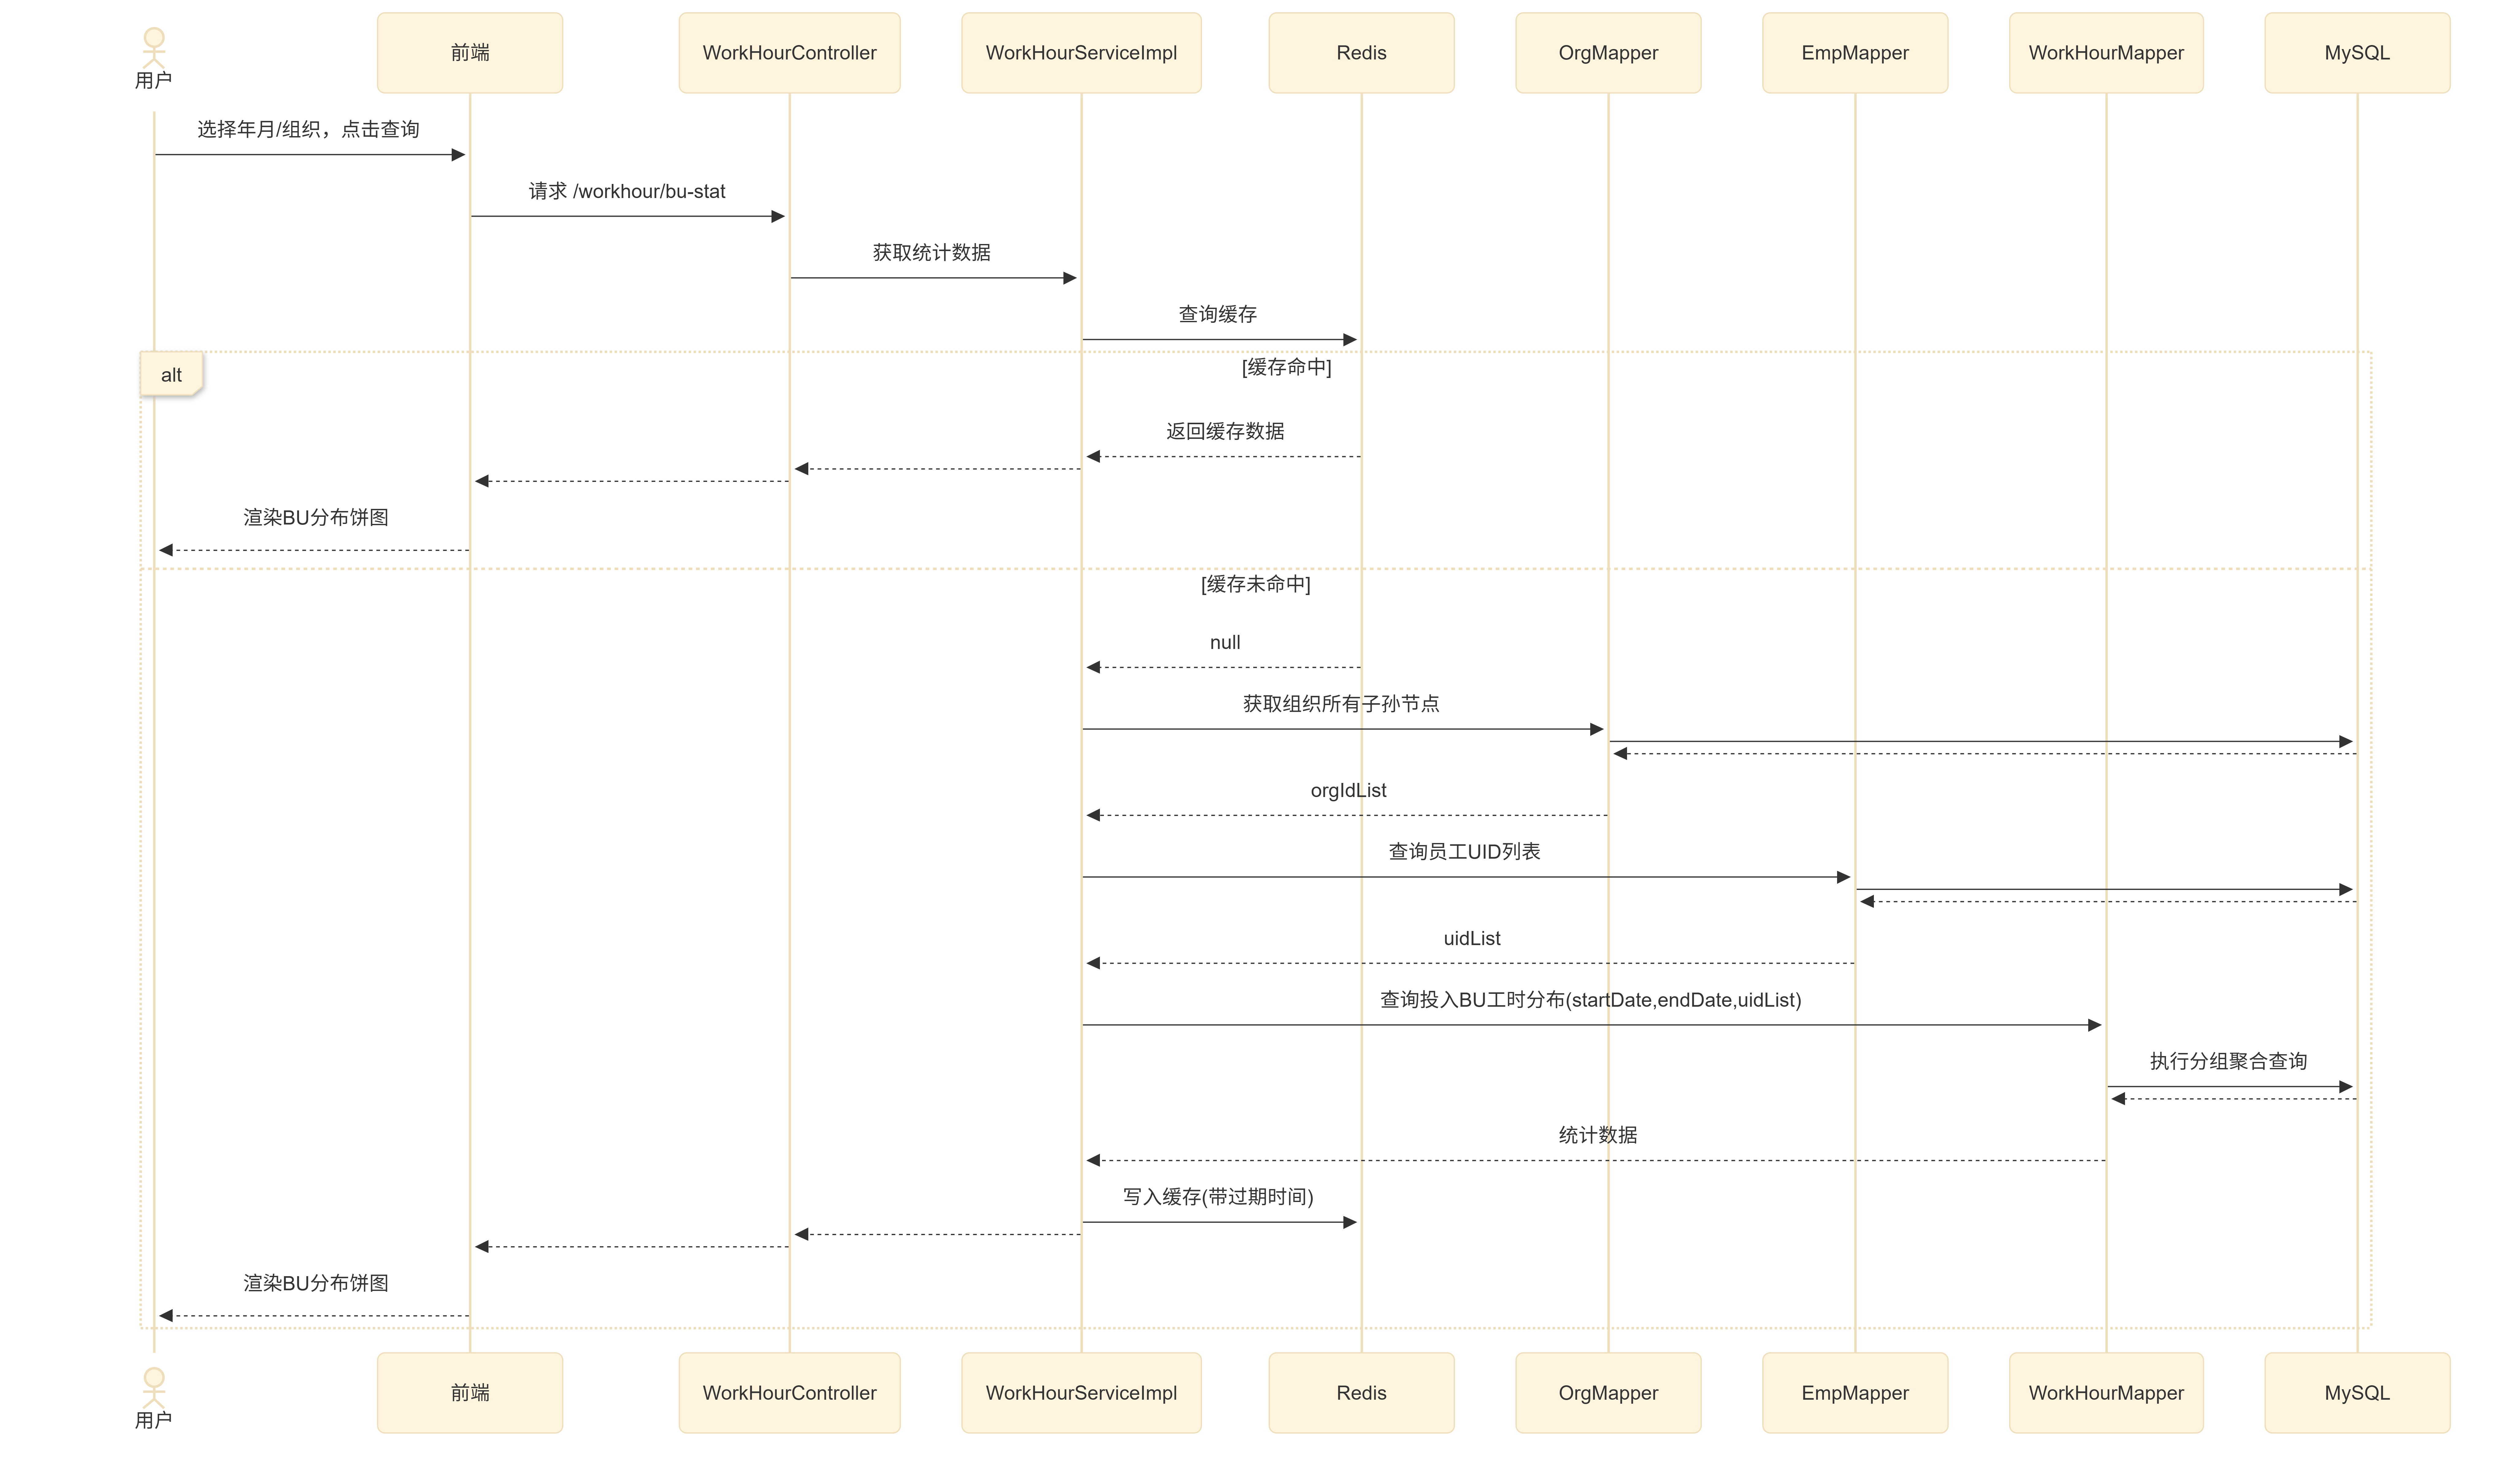
\includegraphics[width=1.0\linewidth]{imgs/Seq/BU工时饼图时序图.png}
	\caption{BU工时饼图时序图}
	\label{fig:seq-bu-hour-distribution}
\end{figure}
用户在前端的下拉框中选择查询的年月和组织节点后，点击查询按钮发起请求。后端请求处理层接收到请求后，首先对参数进行非空和有效性校验，校验通过后进入业务层，首先查询Redis中是否存在对应的图表缓存数据，若命中则直接返回，以此降低到达数据库的请求数量。若缓存未命中，系统首先调用 OrgMapper 递归获取目标组织及其所有子节点的 ID 集合，随后通过 EmployeeMapper 查询出这些节点下所有员工的 UID 列表。同时，针对前端传递的年月参数，考虑到数据库工时表记录的日期精确到天，为避免在 SQL 语句中使用日期格式化函数（如 DATE\_FORMAT）匹配从而引发索引失效问题，业务层会预先将年月参数转换为该月的起止时间范围（即月初第一天至月末最后一天）。接着，将时间参数和 UID 列表传入 WorkHourMapper，调用接口对数据库执行分组聚合查询，计算出各个BU的工时分布情况。最后，系统将该计算结果写入 Redis 并设置过期时间，过期策略是当月数据一小时，其余时间24小时，将数据封装后返回给前端，利用Echarts组件来渲染分布饼图。

用户如果想知道某个BU的工时详情，可以点击对应模块，其核心时序如图\ref{fig:seq-bu-hour-detail}所示。
\begin{figure}[htbp]
	\centering
	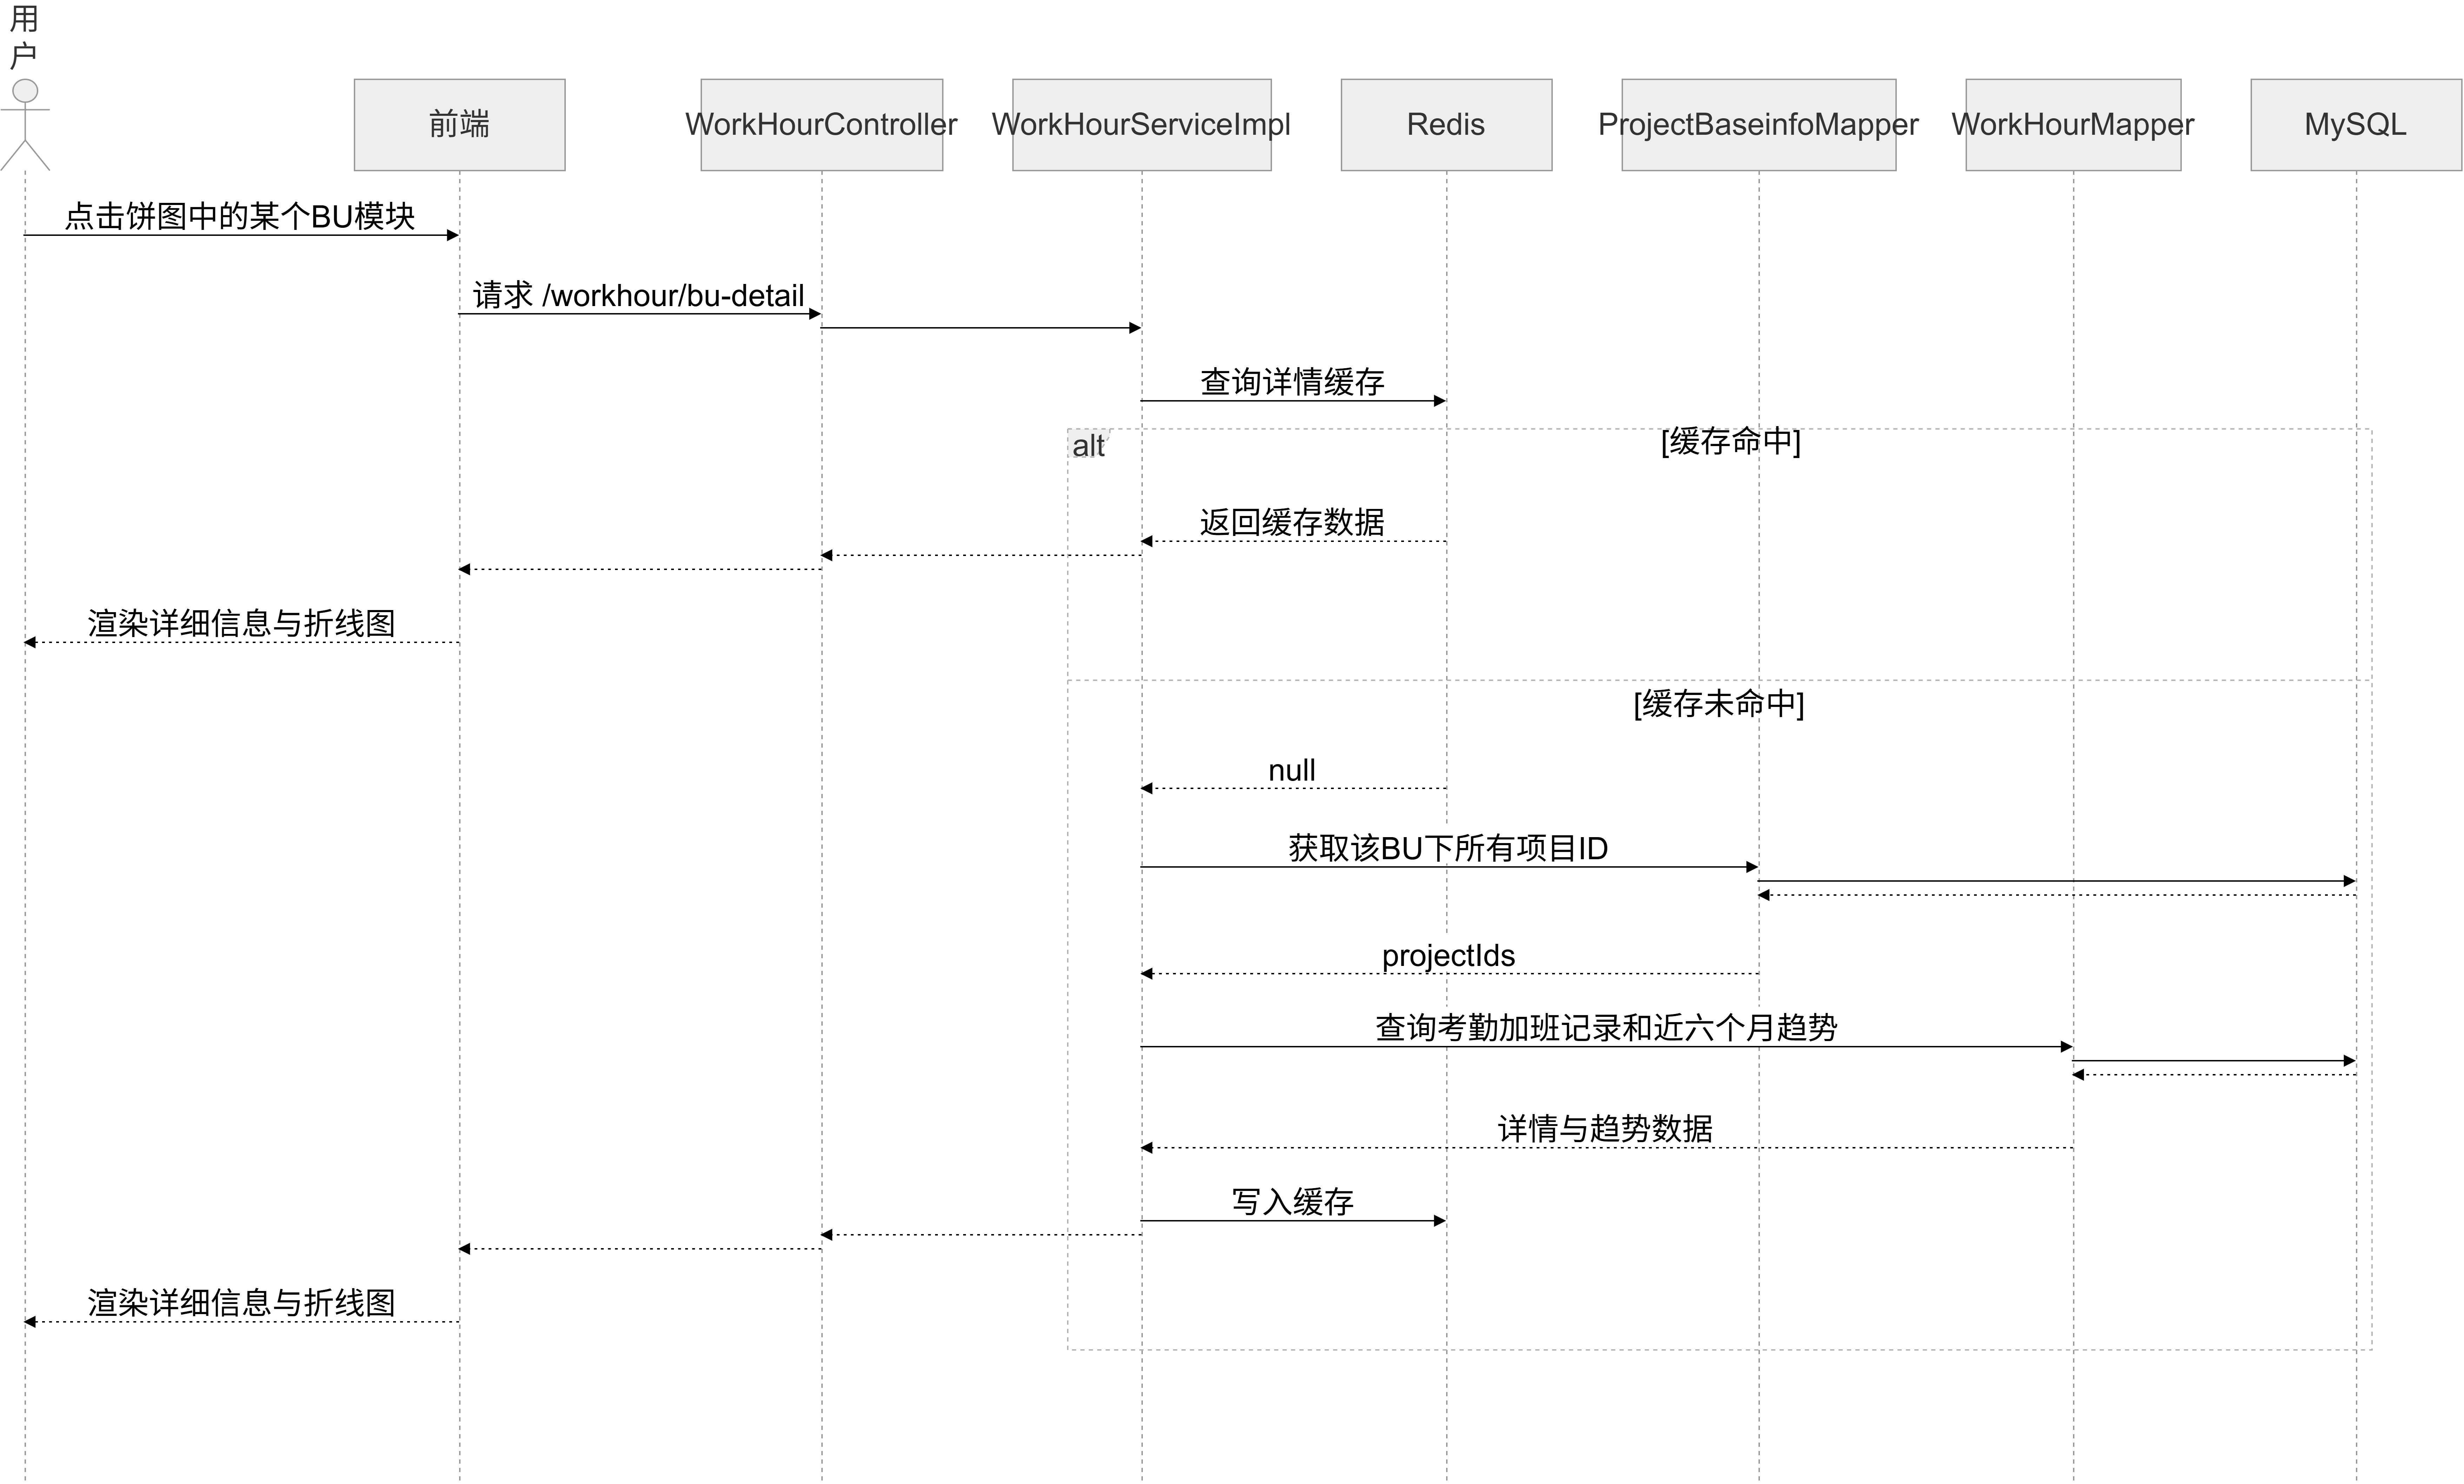
\includegraphics[width=1.0\linewidth]{imgs/Seq/BU详情时序图.png}
	\caption{BU详情时序图}
	\label{fig:seq-bu-hour-detail}
\end{figure}
前端会发起对该 BU 的详情查询请求。后端同样优先进行缓存校验。若缓存未命中，系统首先通过 ProjectMapper 查询出该 BU 下挂载的所有项目 ID 列表。随后，依据项目 ID 调用 WorkHourMapper 查询这些项目的加班工时数和近六个月的工时变化趋势。在将详情数据回写至 Redis时，系统对过期时间进行了抖动处理，以防止大量缓存同时失效引发缓存雪崩问题。数据返回前端后，渲染生成具体的基础信息面板与工时趋势折线图。

\subsection{项目基本信息管理}
项目基本信息维护是玄武平台数字化项目管理部分的一部分。通过该模块，项目经理（SPM）能够对项目的基本信息、里程碑节点及近期交付计划进行统一维护。整个模块的操作主要可划分为基础数据维护与交付节点的高频更新两大维度。

项目基本信息管理类图如图\ref{fig:class-project-baseinfo}所示。
\begin{figure}[htbp]
	\centering
	
\includegraphics[width=1.0\linewidth]{imgs/class/项目基本信息管理类图.png}
	\caption{项目基本信息管理类图}
	\label{fig:class-project-baseinfo}
\end{figure}
在实际开发中，我在 TbProjectBaseinfoController 中定义所有的HTTP接口。对于数据查询操作，使用封装好的 ProjectQueryRequest 参数查询类来接收前端传递的参数，这个类是基类 QueryRequest 的子类，核心的业务逻辑由 TbProjectBaseinfoServiceImpl 承担。内部包含分页查询、新增项目、更新项目、查看更改历史等方法，TbProjectBaseinfoMapper 和 TbProjectBaseinfoHistoryMapper 分别用来与项目基本信息表、项目历史信息表和项目交付历史表进行交互。

其核心业务流转如图\ref{fig:seq-project-baseinfo}所示。
\begin{figure}[htbp]
	\centering
	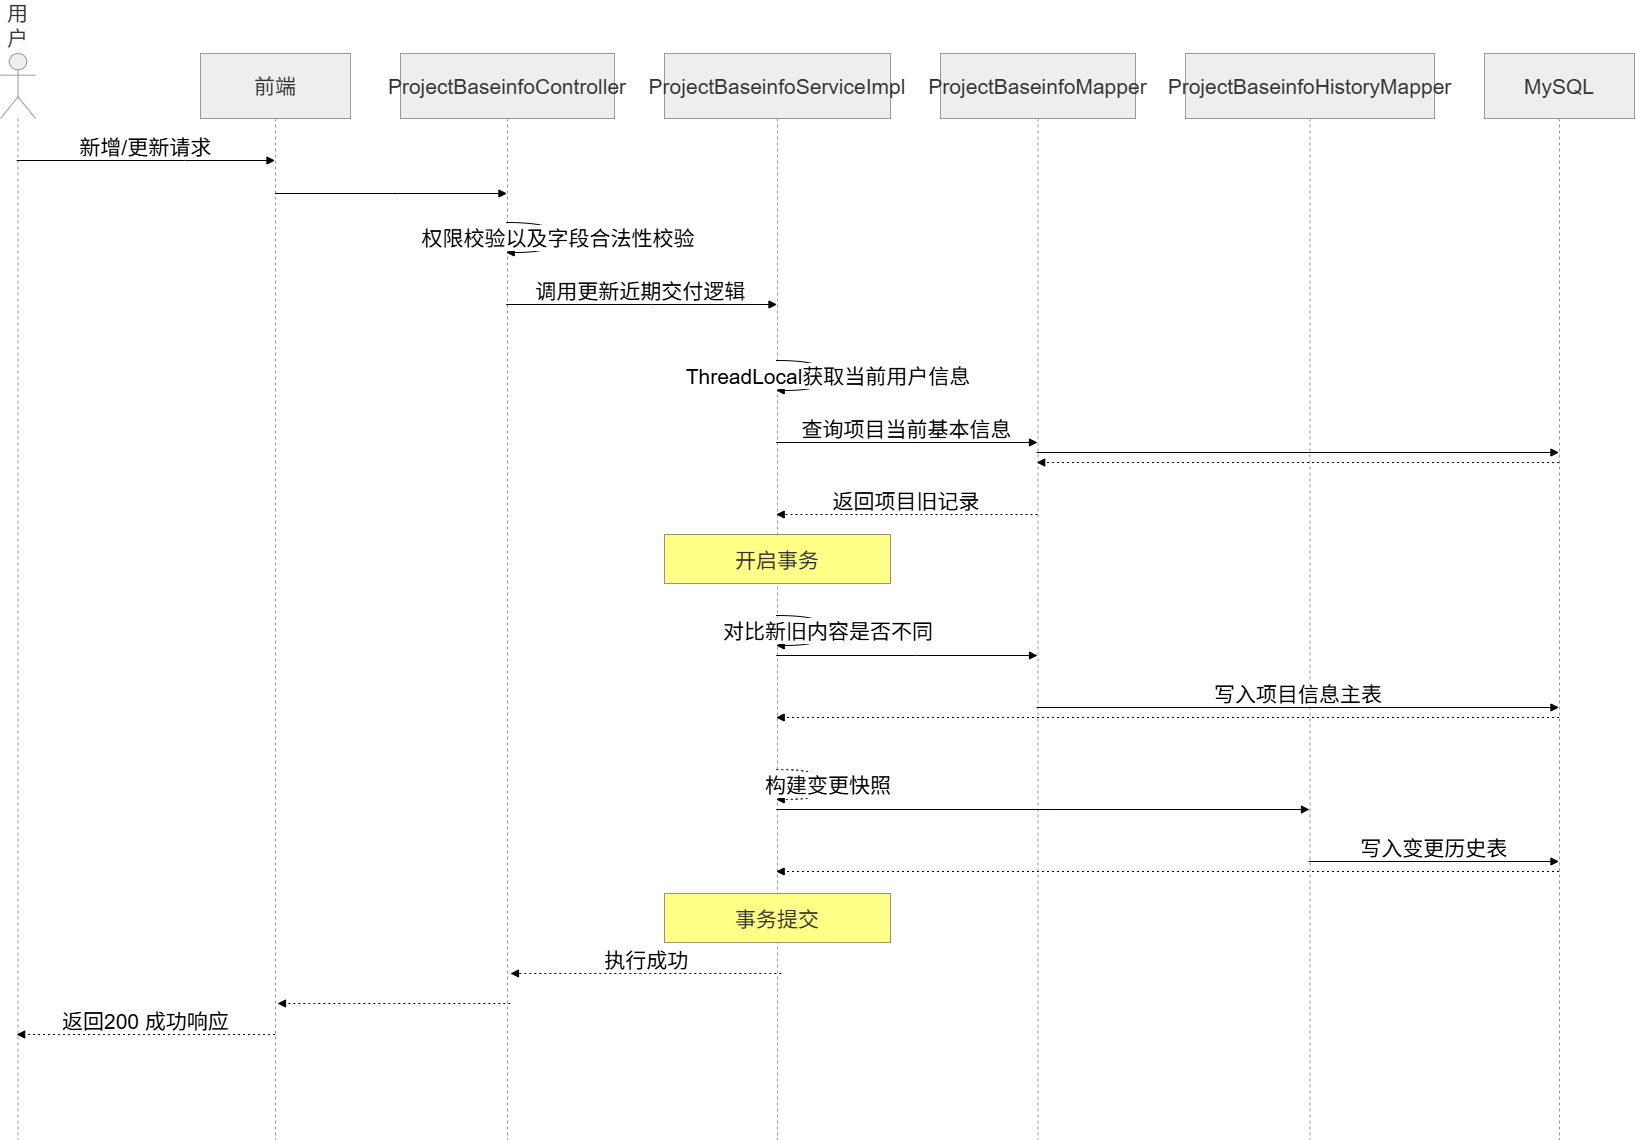
\includegraphics[width=1.0\linewidth]{imgs/Seq/项目信息管理时序图.png}
	\caption{项目信息管理时序图}
	\label{fig:seq-project-baseinfo}
\end{figure}
针对项目基本信息的“新增与更新”流程，系统在后端实现上重点保障了数据的安全性与可追溯性。我们在 TbProjectBaseinfoController 的新增和更新方法上加上了 @RequiresPermissions 注解，前端发起的 HTTP 请求会先经过请求处理层的 JWT 校验，通过后 Shiro 框架会拦截加了注解的方法，在方法执行前先查询预热到缓存的权限数据，如果没有就去数据库查询，检查当前用户是否有对应权限，并利用 \texttt{@Valid} 完成参数的合法性校验。进入业务层后，系统采用“主表+历史表”的双写策略：首先将最新的项目信息更新至MySQL主表；随后，通过构建当前操作的完整数据快照（涵盖新旧值、操作人及操作类型），并写入项目信息快照表。这种快照机制便于后续的项目审计与数据回滚操作。在执行更新操作后，批量清除 Redis 中关联的失效缓存，这样前端在下次查询时能够加载数据库中最新数据。但是由于部分字段比如"近期交付阀点"和"近期阀点日期"修改比较频繁，可能导致快照表的体积变得太大，因此针对这部分的修改历史保存到交付历史变更表中。由于修改了多张表，需要在方法上加上 @Transactional 注解，将多表更新操作限制在单一事务中，以确保原子性和一致性。需要注意的是，在实际开发中，并不是在方法上加注解就可以高枕无忧了，事务包裹的范围应该尽可能小，否则可能会导致长事务的出现，很容易耗尽连接池导致数据库崩溃，同时长期持有的锁会引发大范围阻塞，并因阻碍日志清理而拖垮数据库性能。此外还要考虑注解失效的情景，避免在开发中犯这类错误。

\subsection{缺陷管理}
企业软件项目在研发过程中不可避免地会出现Bug，由于企业实际开发过程中同时使用了多套缺陷跟踪平台，包括Trinity、Jira 和 Bugclose，各平台的缺陷字段各不相同，缺陷管理模块需要对这些缺陷进行统一管理，聚合统计。通过数据汇聚与指标计算，为项目质量人员提供多维度的缺陷质量看板。

缺陷管理类图如图\ref{fig:class-bug}所示。
\begin{figure}[htbp]
	\centering
	
\includegraphics[width=1.0\linewidth]{imgs/class/缺陷管理类图.png}
	\caption{缺陷管理类图}
	\label{fig:class-bug}
\end{figure}
在这个部分定义了 BugQueryRequest 查询类，作为 QueryRequest 的子类，内部设置了自定义的条件过滤器集合，便于对多个字段进行多种条件筛选，业务处理层是该模块的计算核心。BugServiceImpl 注入了 BugMapper 来执行缺陷表的查询操作。BugServiceImpl 还注入了 ProjectClusterService，在处理“项目聚类统计汇总”这一业务时，能调用其中的方法来获取所有聚类名称或者根据聚类名称查询该聚类下的所有挂载项目清单。

（1）项目聚类缺陷统计

缺陷管理部分主要包括缺陷数据的分页查询以及项目聚类缺陷统计，其中，项目聚类缺陷统计的业务流程如图\ref{fig:seq-bug-cluster}所示。
\begin{figure}[!htbp]
	\centering
	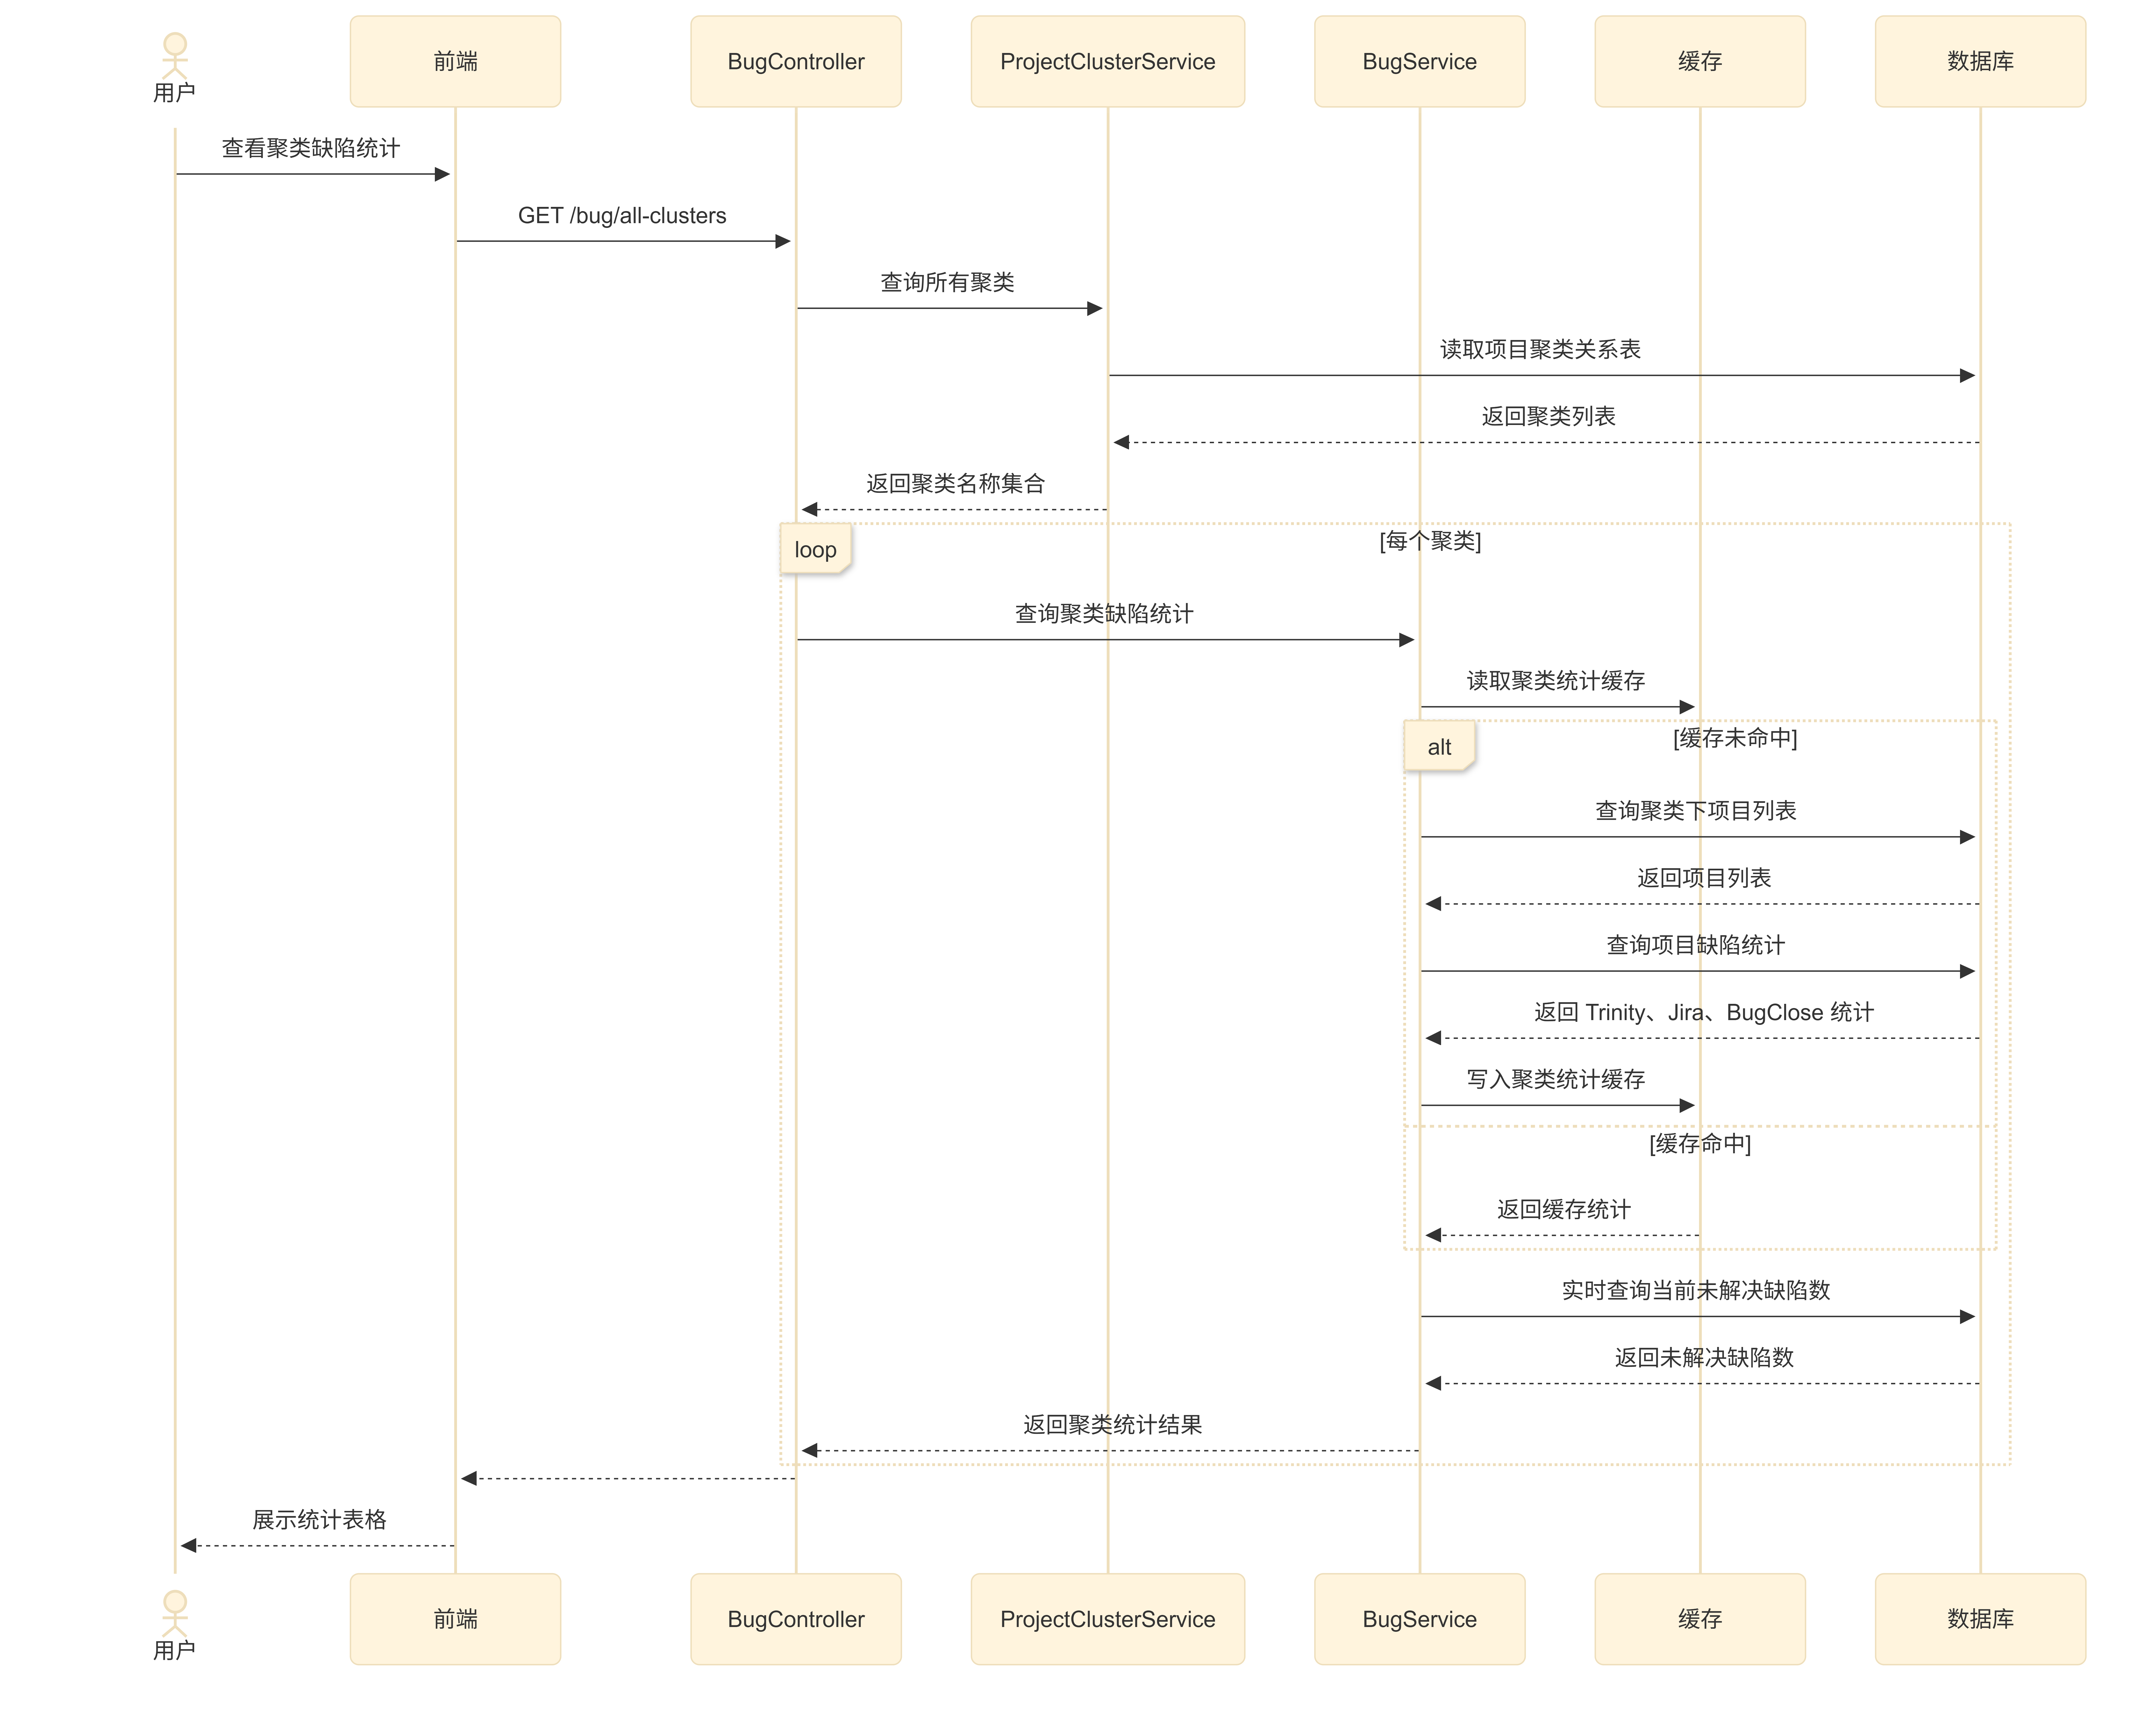
\includegraphics[width=1.0\linewidth]{imgs/Seq/项目聚类缺陷统计时序图.png}
	\caption{项目聚类缺陷统计时序图}
	\label{fig:seq-bug-cluster}
\end{figure}
项目聚类缺陷统计主要用于对多个项目组成的聚类进行缺陷数据汇总分析。系统首先从项目聚类关系表中获取全部聚类名称，并根据聚类名称查询其包含的项目列表。随后，系统以项目为基本统计单元，分别从 Trinity 缺陷表、Jira 缺陷表和 BugClose 缺陷表中提取缺陷数据，并计算当前未解决缺陷数、新增缺陷数、解决缺陷数、超期未解决缺陷数以及关闭率等指标。最后以表格的形式展示给用户，对于一些关闭率低的项目聚类，还设置了定时任务发送飞书预警消息来提醒。

考虑到聚类缺陷统计涉及多个数据表，查询成本较高，系统在设计中引入缓存机制。对于昨日新增、昨日解决、总缺陷数、关闭数以及聚类级历史统计等变化频率较低的数据，系统使用缓存保存统计结果；对于当前未解决缺陷数等实时性要求较高的数据，则在接口调用时进行实时计算，并与缓存结果合并后返回。该设计在保证统计结果实时性的同时，降低了数据库访问压力，提高了聚类缺陷看板的响应效率。

（2）缺陷数据深分页优化

系统的缺陷数据来自于三个外部平台（Trinity,Jira,BugClose），分别存储至数据库的三张同步表（"tb\_sync\_bug"、"tb\_sync\_jira"、"tb\_sync\_bugclose"），然后在前端进行分页查询。由于缺陷数据表的体积非常大，无论是进行分页查询还是excel导出时都会出现较大的延迟。excel导出由于内存里放不下这么多数据，可以参考外部排序的思想，利用游标来分批获取数据并写入Excel。对于深分页，出现这个问题的原因是因为对于 LIMIT offset, N，MySQL 并非直接跳到 offset 处，而是必须从头扫描 offset + N 条记录。如果查询依赖二级索引且不满足覆盖索引，这意味着 MySQL 需要对前 offset 条记录执行毫无意义的回表查询（产生海量的随机 I/O），最后再将这些辛苦查出的数据丢弃。即便优化器最终因代价过高退化为全表扫描，顺序扫描百万行的成本依然巨大。对于分页查询来说，我们可以通过延迟关联将 LIMIT 操作转移到主键索引树上，减少回表次数，再通过INNER JOIN将子查询结果集成到主查询中。
\begin{figure}[htbp]
	\centering
	\noindent % 消除首行缩进，确保左侧完全对齐
	\begin{minipage}[t]{0.42\textwidth}
		\textbf{优化前（传统单表分页）}
		\begin{lstlisting}[language=SQL, frame=single, basicstyle=\ttfamily\small, breaklines=true, tabsize=4]
			SELECT * FROM tb_sync_bug
			WHERE severity = 'A'
			ORDER BY created_date DESC
			LIMIT 100000, 20
		\end{lstlisting}
	\end{minipage}
	\hfill
	\begin{minipage}[t]{0.54\textwidth}
		\textbf{优化后（延迟关联分页）}
		\begin{lstlisting}[language=SQL, frame=single, basicstyle=\ttfamily\small, breaklines=true, tabsize=4]
			SELECT b.* FROM tb_sync_bug b
			INNER JOIN (
			SELECT id, created_date FROM tb_sync_bug
			WHERE severity = 'A'
			ORDER BY created_date DESC, id ASC
			LIMIT 100000, 20
			) page_ids ON page_ids.id = b.id
			ORDER BY page_ids.created_date DESC, page_ids.id ASC
		\end{lstlisting}
	\end{minipage}
	\caption{深分页优化前后 SQL 语句横向对比}
	\label{fig:sql-optimization-compare}
\end{figure}

\subsection{重大问题管理}
% 模块功能设计
重大问题管理模块面向项目执行过程中影响范围较大、处理周期较长或需要跨部门协调的问题，大致可分为问题登记、问题处理和问题关闭三个阶段。具体流程如图\ref{fig:serious-problem-process}所示。
\begin{figure}[htbp]
	\centering
	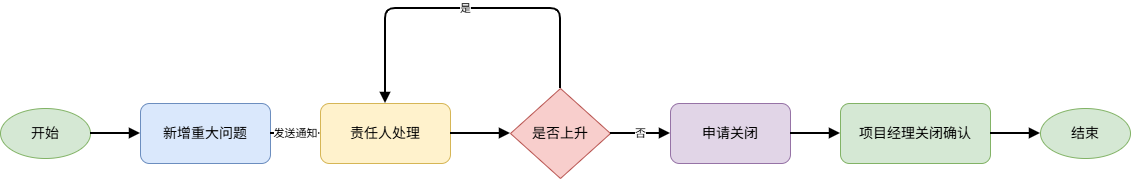
\includegraphics[width=1.0\linewidth]{imgs/Flowchart/重大问题流程图.drawio.png}
	\caption{重大问题流程图}
	\label{fig:serious-problem-process}
\end{figure}

重大问题管理类图如图\ref{fig:class-serious-problem}所示。
\begin{figure}[htbp]
	\centering
	
\includegraphics[width=1.0\linewidth]{imgs/class/重大问题管理类图.png}
	\caption{重大问题管理类图}
	\label{fig:class-serious-problem}
\end{figure}
这部分功能主要围绕实体类 TbProjectSeriousProblem 展开，在控制层提供了分页查询，新增/更新，导出excel以及发送飞书提醒消息的功能，到了业务层，可以通过员工服务ITbEmpBaseinfoService的相关接口补全关联项目与干系人的元数据；其次，发送飞书消息时需要根据重大问题是否上升处理来调整接收人列表，通过调用OrgService的fetchOrgLeaderByOrganCode() 方法在组织树中向上递归溯源，精准定位并提取根因部门的组织负责人信息，最后将组织好的上下文交给IFeishuService，利用其 sendTemplateCard() 方法渲染为飞书消息卡片并发送。

重大问题管理的核心业务流程如图\ref{fig:seq-serious-problem}所示。用户进入列表页面后，系统首先根据当前登录用户的身份判断其权限，查询并展示其可见的问题记录。用户可通过顶部筛选栏按多维度条件进行检索，也可点击"新增"按钮创建新的重大问题。
\begin{figure}[!htbp]
	\centering
	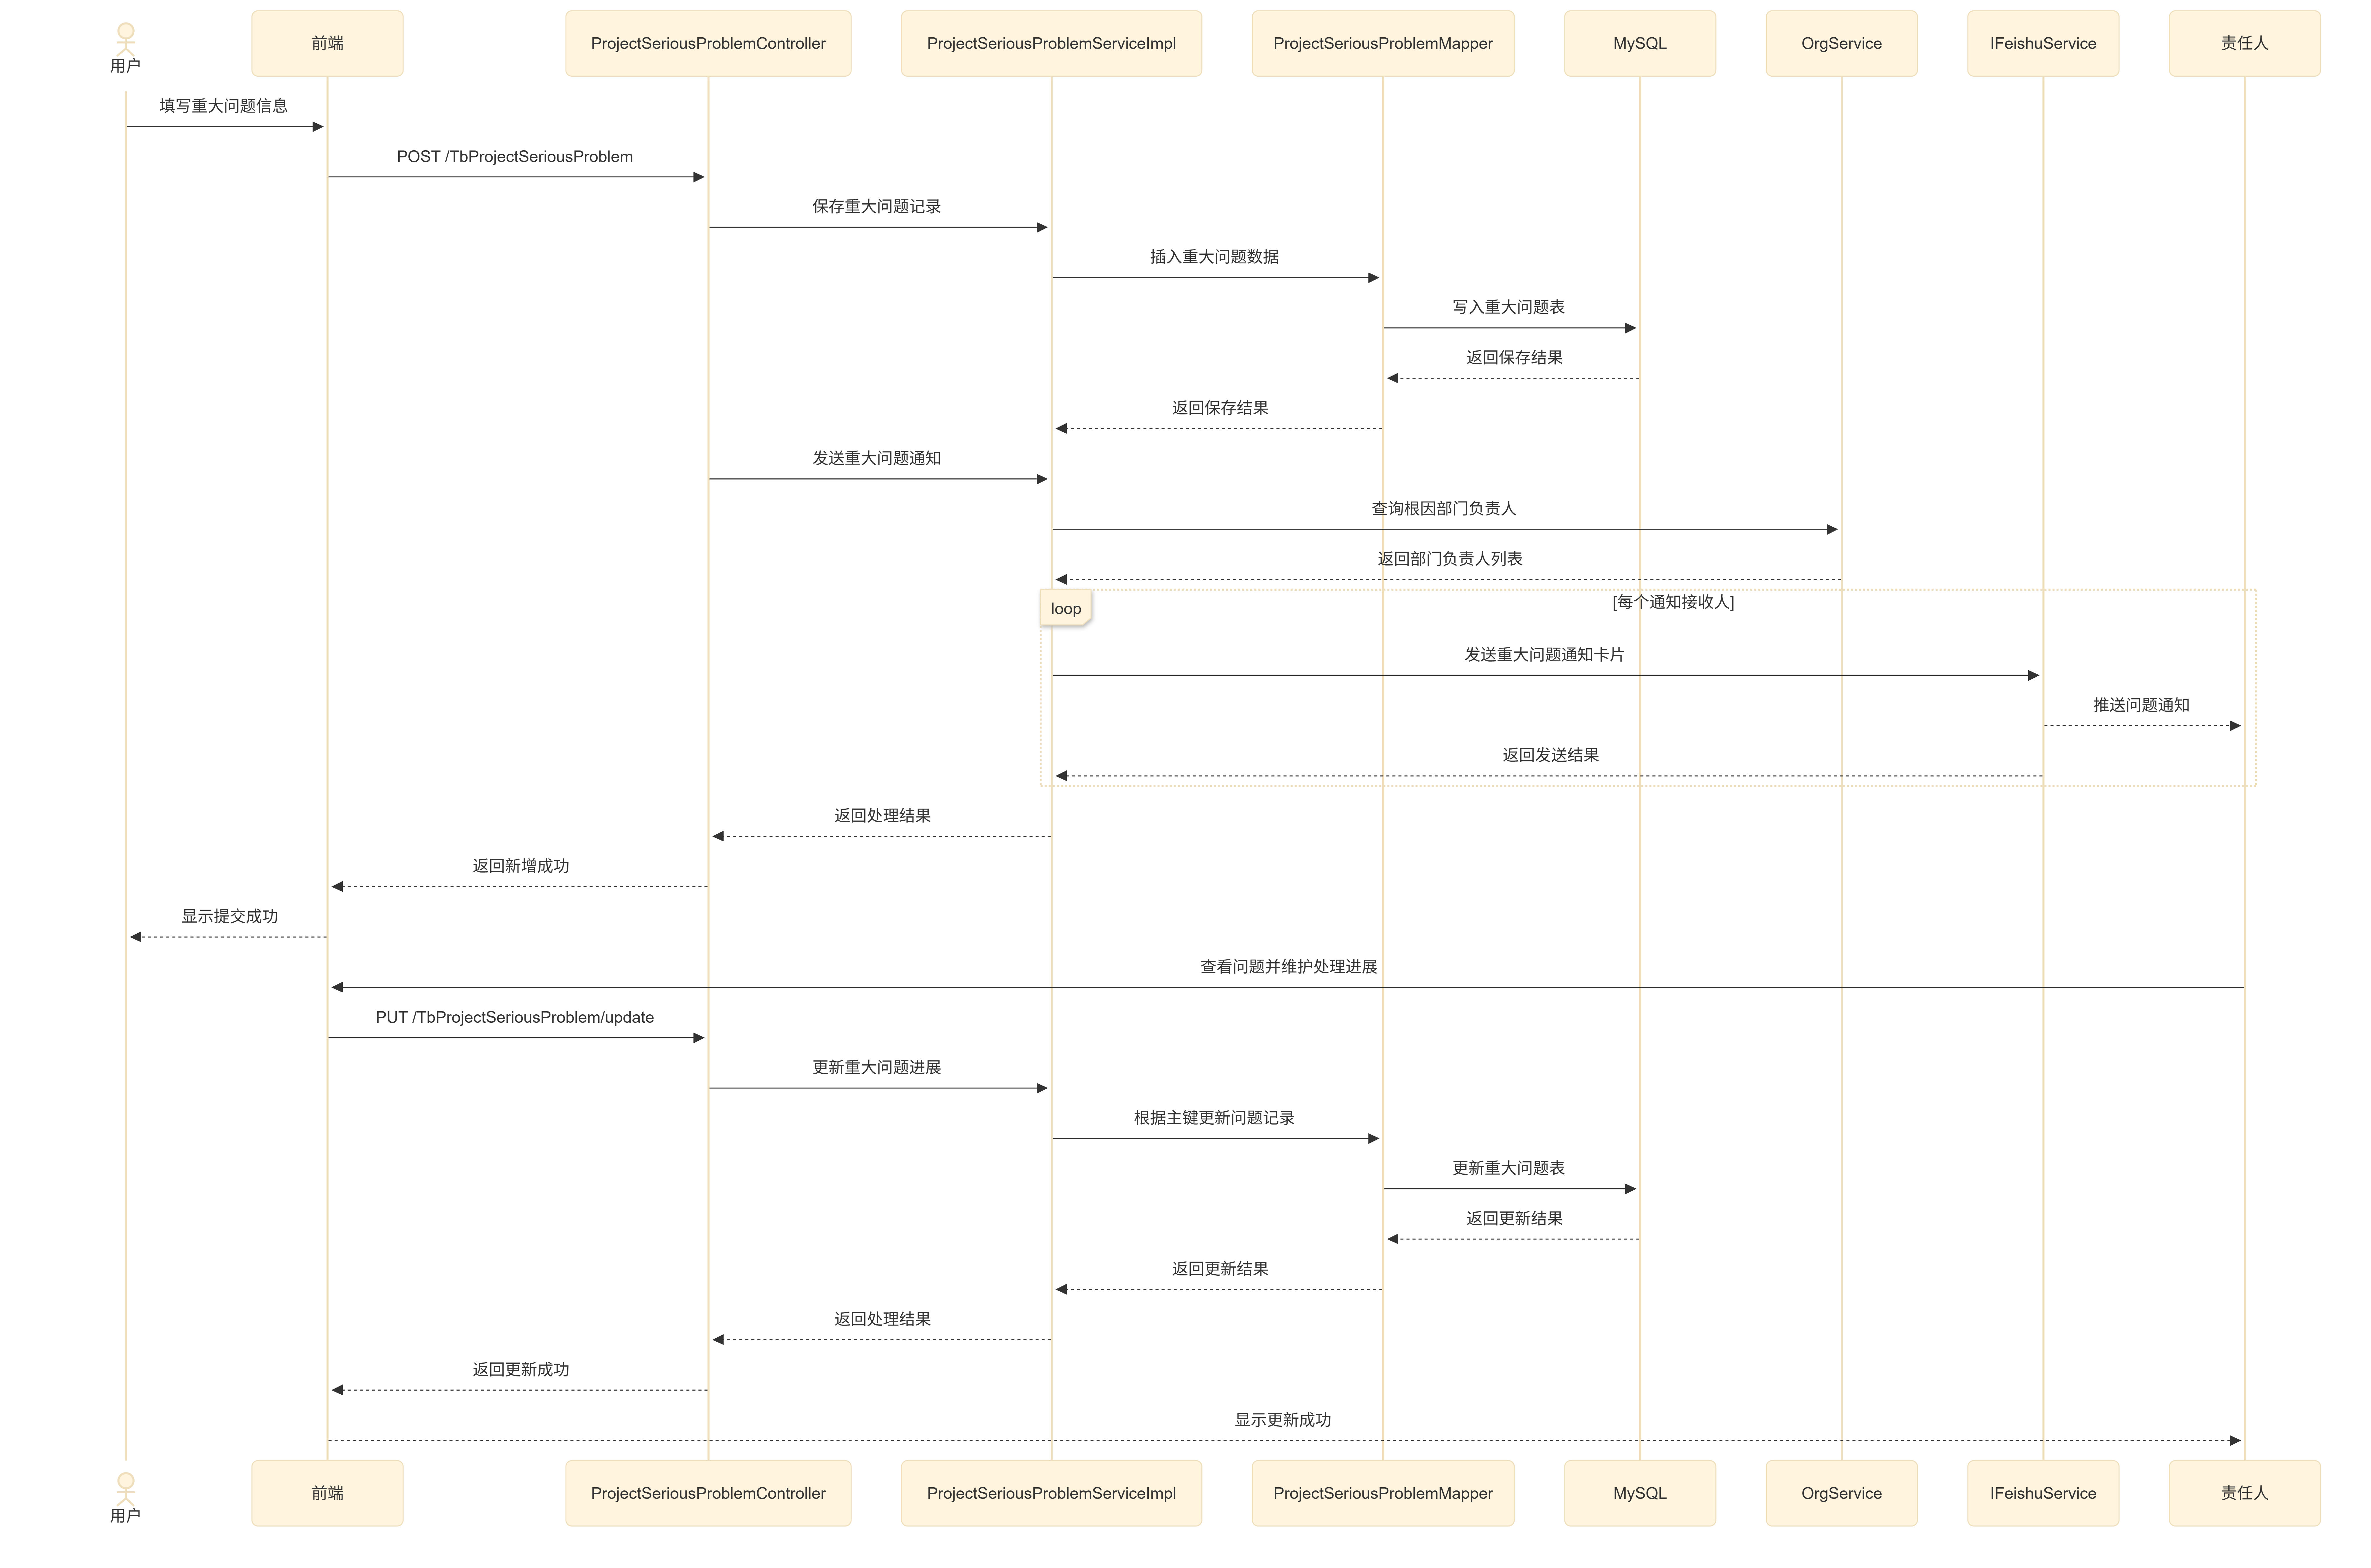
\includegraphics[width=1.0\linewidth]{imgs/Seq/重大问题时序图.png}
	\caption{重大问题时序图}
	\label{fig:seq-serious-problem}
\end{figure}

在问题登记阶段，用户填写重大问题的基础信息和首问闭环责任人。系统保存记录后，根据问题涉及的责任人生成通知内容，并通过飞书消息推送给相关人员，使问题能够及时进入处理环节。在问题处理阶段，由责任人来填写问题的技术原因和解决方案；当问题需要更高层级协调时，可将问题标记为“需要上升”，并指定上升责任人，由其介入协调资源后继续推进问题处理。当问题需要关闭时，用户需要补充实际解决日期、最终责任人、责任分类、技术原因、技术解决方案等信息。系统根据计划解决日期和实际解决日期自动判断问题状态：实际解决日期不晚于计划解决日期时，问题状态为按时关闭；实际解决日期晚于计划解决日期时，问题状态为超期关闭；若超过计划解决日期仍未填写实际解决日期，则问题保持超期未关闭状态。通过该设计，模块能够对重大问题从发现、处理、上升到关闭的全过程进行记录和约束。

\section{数据库设计}
为说明系统中各业务数据对象之间的关系，本文首先给出数据库的总体逻辑 ER 图，如图 \ref{fig:er-overall} 所示。该图从业务对象角度抽象出组织、员工、项目、缺陷、重大问题、项目聚类和聚类缺陷快照等核心实体，并描述各实体之间的主要关联关系。后续小节将在此基础上分别说明关键数据表的字段设计。

\subsection{数据库总体设计}
\begin{figure}[htbp]
	\centering
	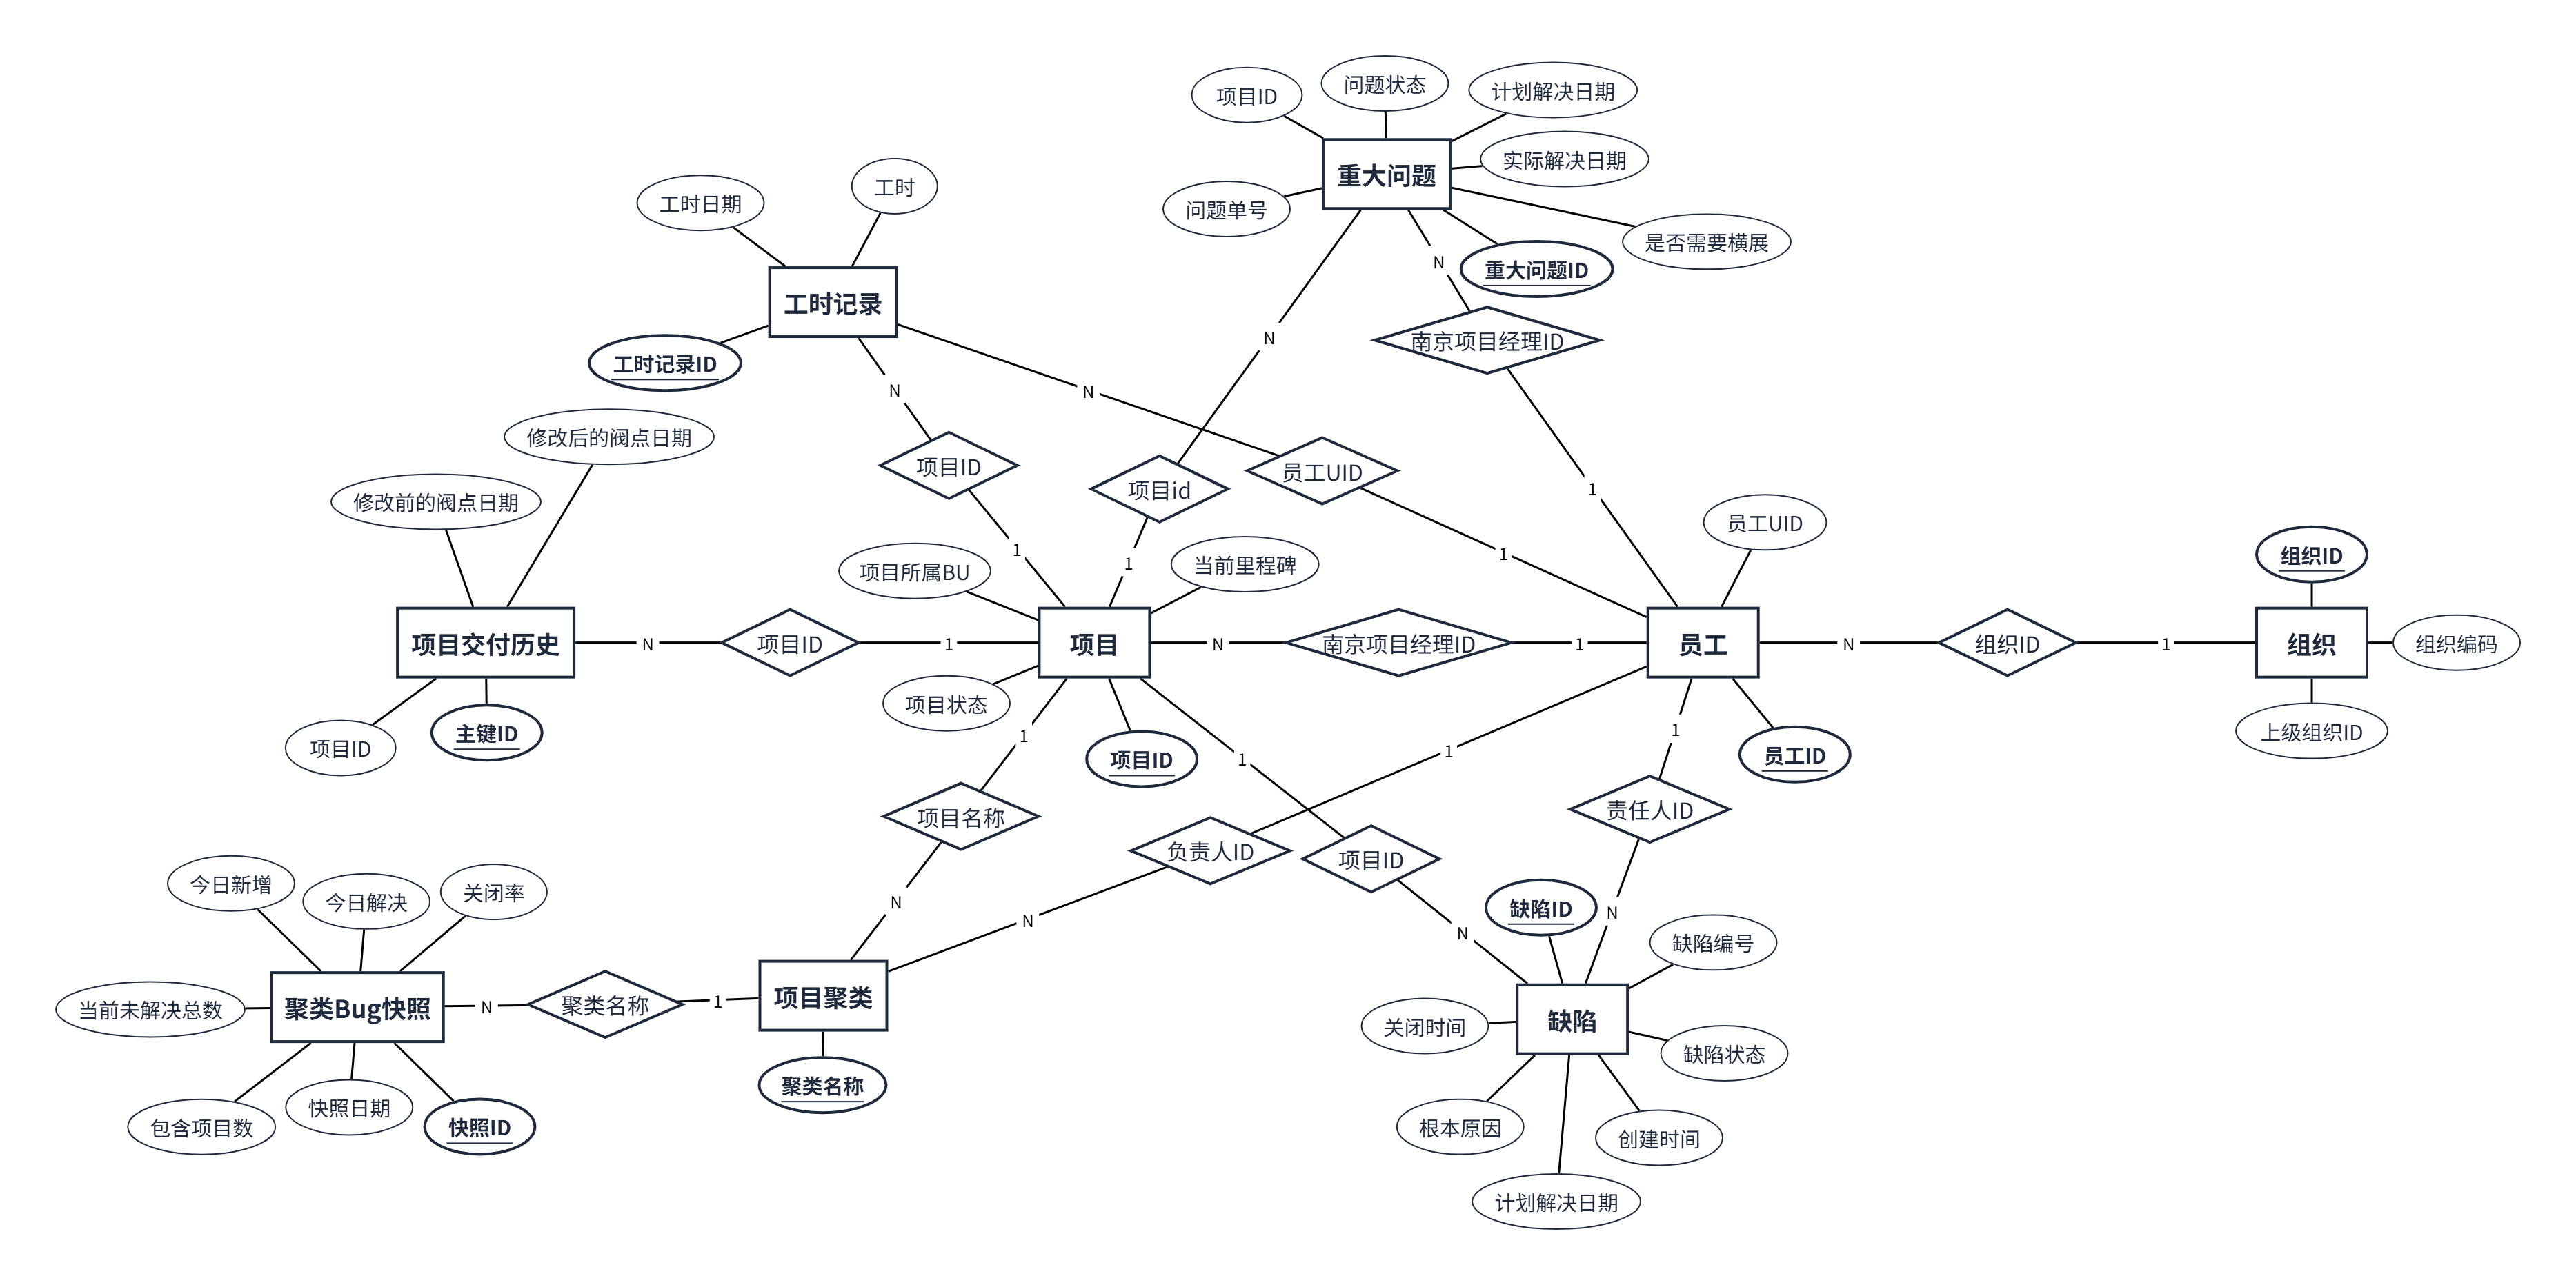
\includegraphics[width=1.0\linewidth]{imgs/ER/er-diagram.png}
	\caption{数据库E-R图}
	\label{fig:er-overall}
\end{figure}
系统数据库以项目为主要业务对象进行组织。项目在系统中既是缺陷统计、工时记录和重大问题管理的归属对象，也是项目聚类分析的基础单元。因此，在总体 ER 图中，项目实体位于业务数据关系的中心位置，并分别与缺陷、重大问题、工时记录、项目交付历史和项目聚类等实体建立联系。

组织和员工实体用于描述系统中的人员基础数据。组织实体记录组织编号、组织编码以及上级组织编号，用于表示企业内部的层级结构；员工实体记录员工编号、员工 UID 以及所属组织。员工与组织之间是一对多关系，即一个组织下可以包含多名员工，而每名员工归属于一个组织。

项目实体记录项目状态、项目所属 BU、南京项目经理、当前里程碑、近期交付阀点及阀点日期等信息。项目与员工之间通过项目经理的id建立关联，一个项目经理可以负责多个项目。项目交付历史实体用于记录项目近期交付的变更情况。该实体与项目实体之间是一对多关系，表示同一项目在执行过程中可能产生多次交付节点调整记录。

缺陷实体用于保存项目缺陷的主要信息。缺陷与项目之间是一对多关系，一个项目可以对应多条缺陷记录；缺陷与员工之间通过责任人建立关联，用于定位缺陷处理人员。

重大问题实体用于记录项目执行过程中需要重点跟踪的问题。重大问题与项目之间是一对多关系，即一个项目可以产生多条重大问题记录。

项目聚类是指将多个相关项目归为一组，以组为单位进行缺陷统计。系统通过聚类名称将若干项目归为同一统计对象，并为聚类配置负责人。项目聚类与项目之间形成一对多关系，一个聚类可以包含多个项目；项目聚类与员工之间通过负责人建立关联，用于表示该聚类统计对象的管理责任人。聚类 Bug 快照与项目聚类之间是一对多关系，同一聚类可以按日期保存多条快照记录，从而支持缺陷趋势分析。

总体来看，该数据库模型以项目为中心，将人员组织、缺陷数据、重大问题、工时记录、交付历史和聚类统计数据连接起来。组织和员工实体提供人员归属关系，项目实体承载项目基础信息，缺陷和重大问题实体记录项目执行过程中的质量问题，项目聚类和聚类 Bug 快照实体则面向跨项目统计分析。由于部分业务数据来源于外部同步表，实际物理表中并非所有关系都采用数据库外键约束，图中的关系主要用于描述系统业务对象之间的逻辑关联。

\subsection{数据表结构设计}
\begin{enumerate}[label=(\arabic*)]	
	\item BU工时统计主要用于分析各个组织部门在业务单元的工时投入情况，涉及的实体包括组织树（\texttt{tb\_org\_tree}）、员工基础信息（\texttt{tb\_emp\_baseinfo}）、项目列表（\texttt{tb\_project\_\allowbreak baseinfo\_\allowbreak new}）、工时记录（\texttt{tb\_sync\_wh}）和考勤工时（\texttt{tb\_sync\_attend\_hour}），其关系如图\ref{fig:er-org-wh}所示。
	
	\begin{figure}[htbp]
		\centering
		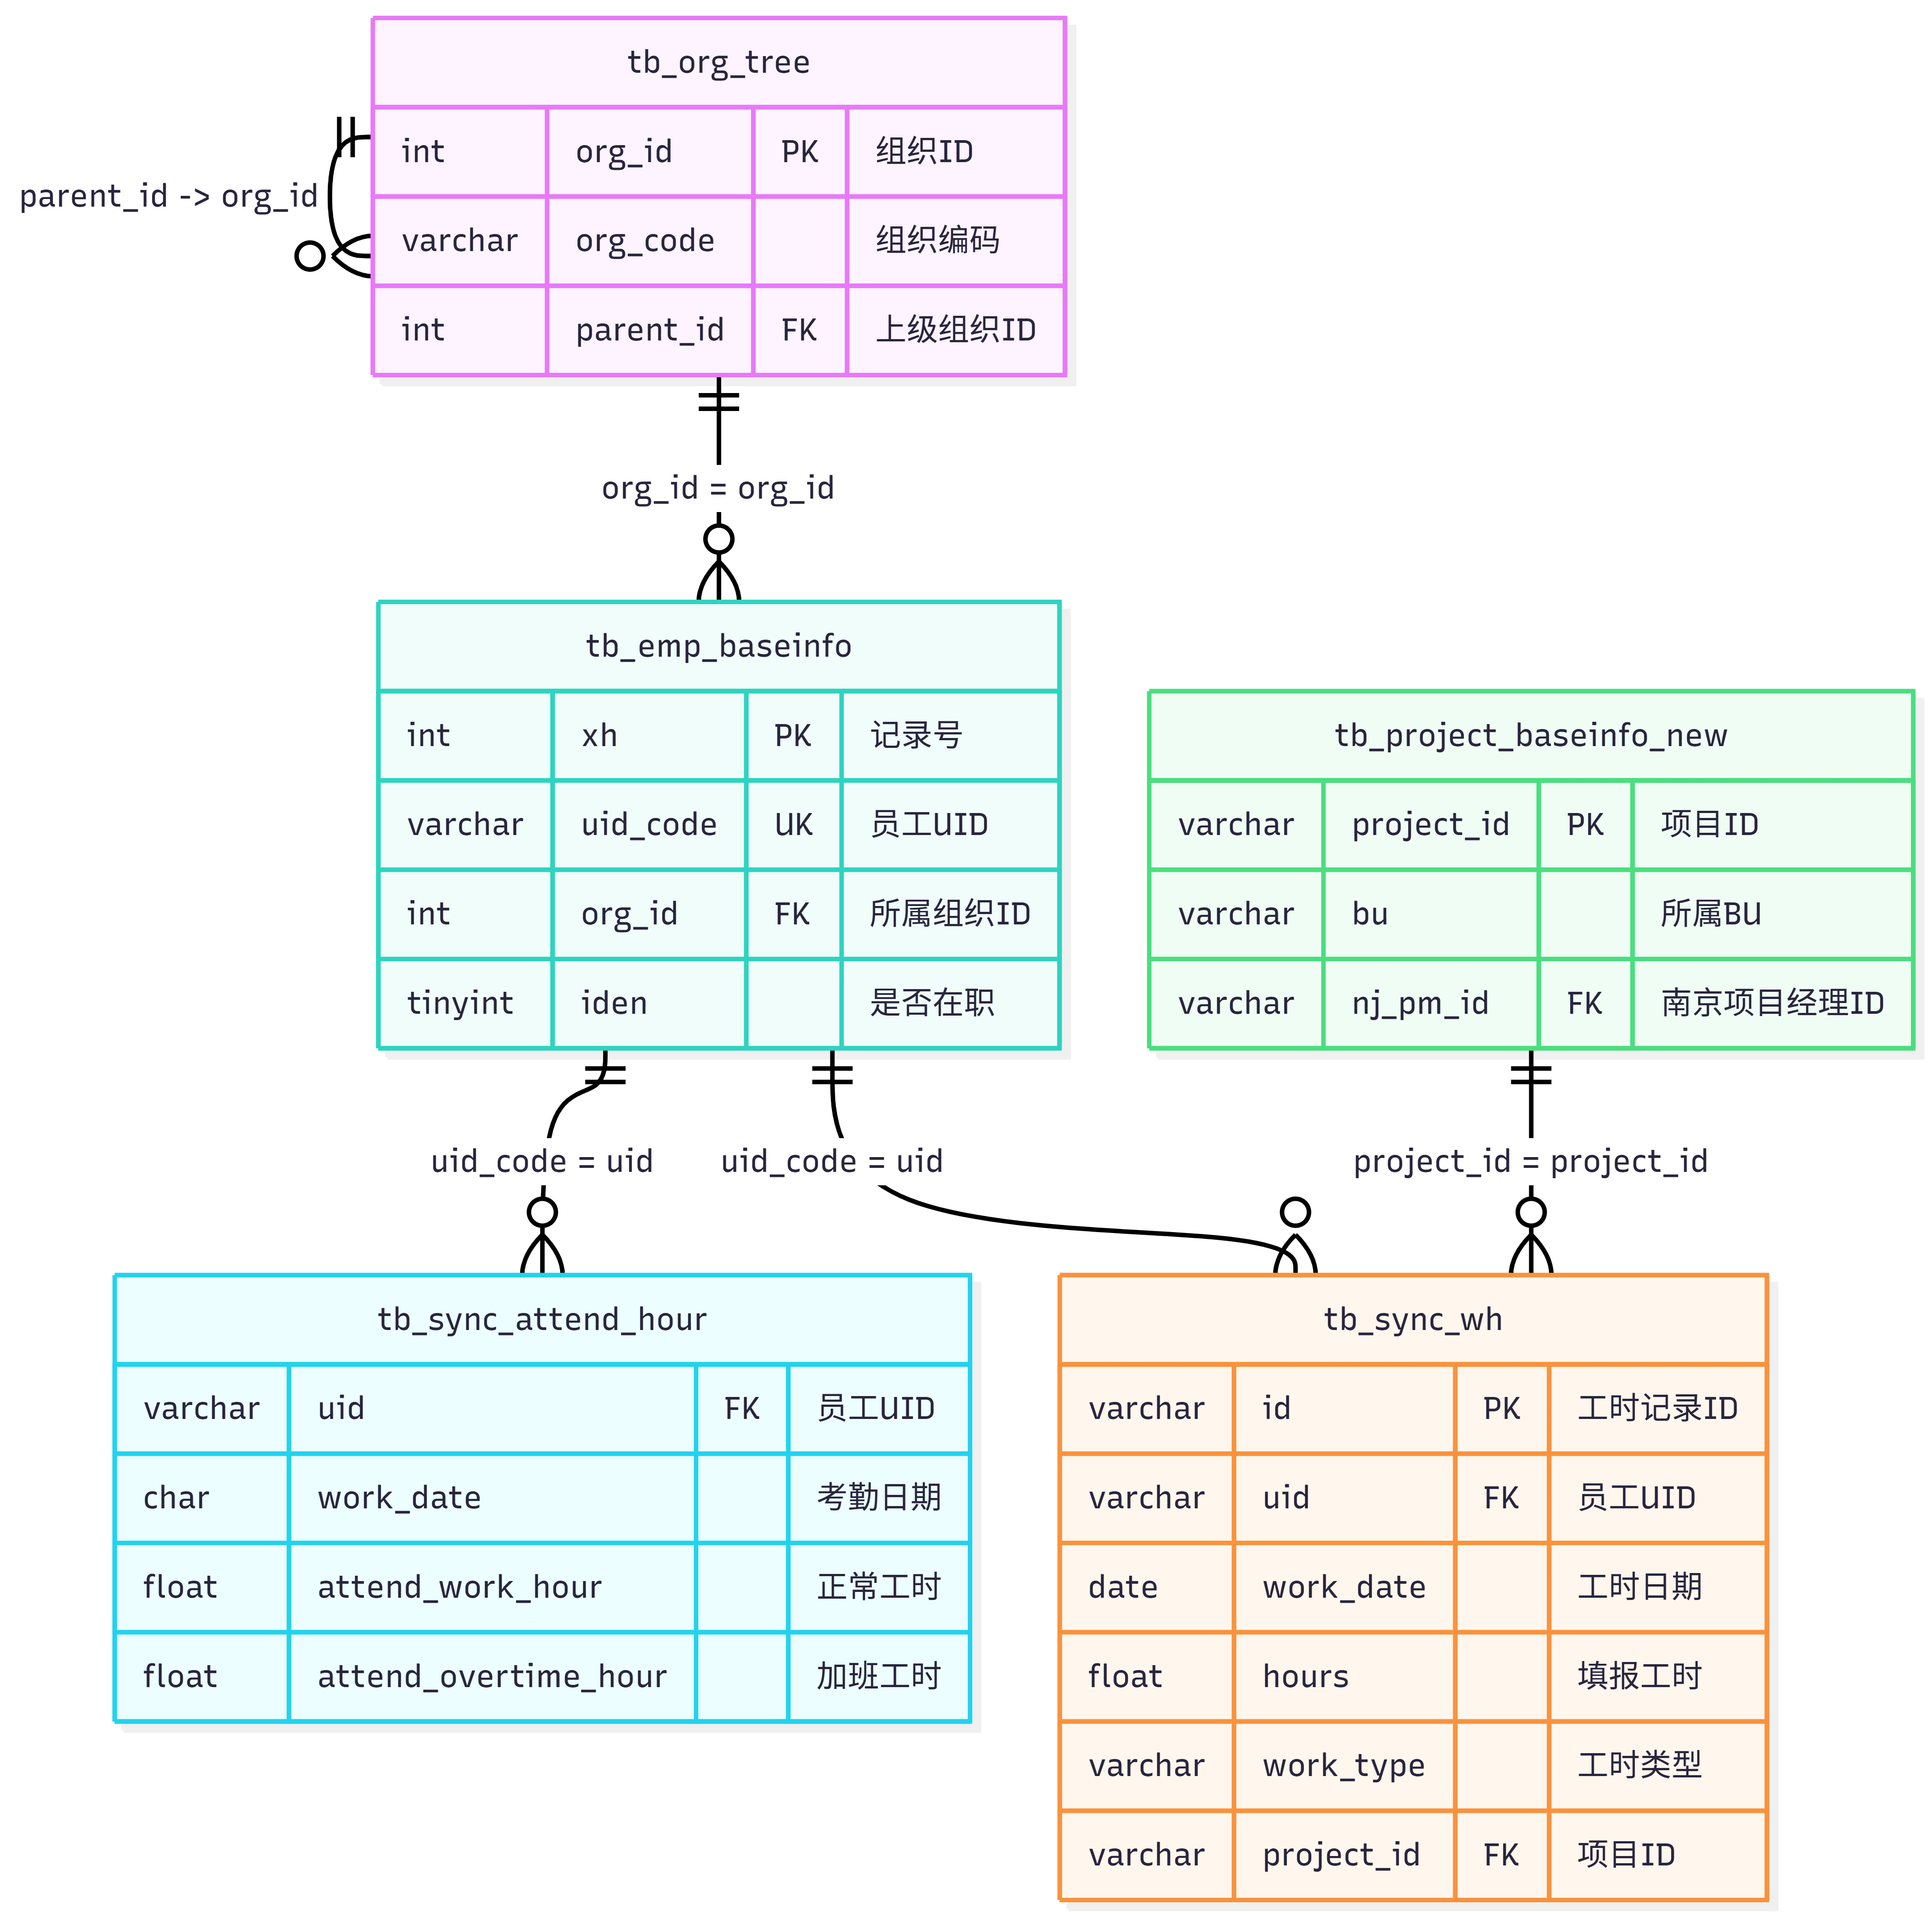
\includegraphics[width=0.7\linewidth]{imgs/ER图-部门投入BU工时分析.png}
		\caption{工时E-R图}
		\label{fig:er-org-wh}
	\end{figure}
	
	在该 E-R 模型中，\verb|tb_org_tree| 用于保存组织树结构，通过 \verb|parent_id| 与 \verb|org_id| 的自关联关系描述组织上下级层级。\verb|tb_emp_baseinfo| 用于保存员工基础信息，其中 \verb|org_id| 表示员工所属组织，\verb|uid_code| 是员工在系统中的唯一标识。工时记录表 \verb|tb_sync_wh| 存储从 Trinity 系统同步而来的员工填报工时数据，通过 \verb|uid| 与员工表中的 \verb|uid_code| 建立逻辑关联，通过 \verb|project_id| 与项目基础信息表中的 \verb|project_id| 建立逻辑关联。考勤工时表 \verb|tb_sync_attend_hour| 保存员工每日考勤工时、加班工时和填写工时等数据，同样通过 \verb|uid| 与员工表关联。
	
	该模型能够支撑 BU 工时趋势分析、BU 加班工时统计和 BU 工时占比分析等功能。系统的接口首先接收年月、组织ID作为参数，根据组织树获取目标部门下的员工范围，然后根据员工范围查询指定时间范围内的工时记录，并结合项目所属 BU 字段完成按 BU 的聚合统计。同时，通过考勤工时表中的加班字段，可以进一步计算某个 BU 的加班投入情况以及近几个月的工时趋势。
	
	\item 项目基本信息管理是项目运营管理模块的基础，其数据模型围绕项目主数据展开，并关联项目交付历史、项目里程碑和项目负责人等信息，涉及的实体包括员工信息、项目基本信息、交付历史（\verb|tb_project_delivery_history|）和里程碑（\verb|tb_project_milestone|），其关系如图\ref{fig:er-project}所示
	
	\begin{figure}[htbp]
		\centering
		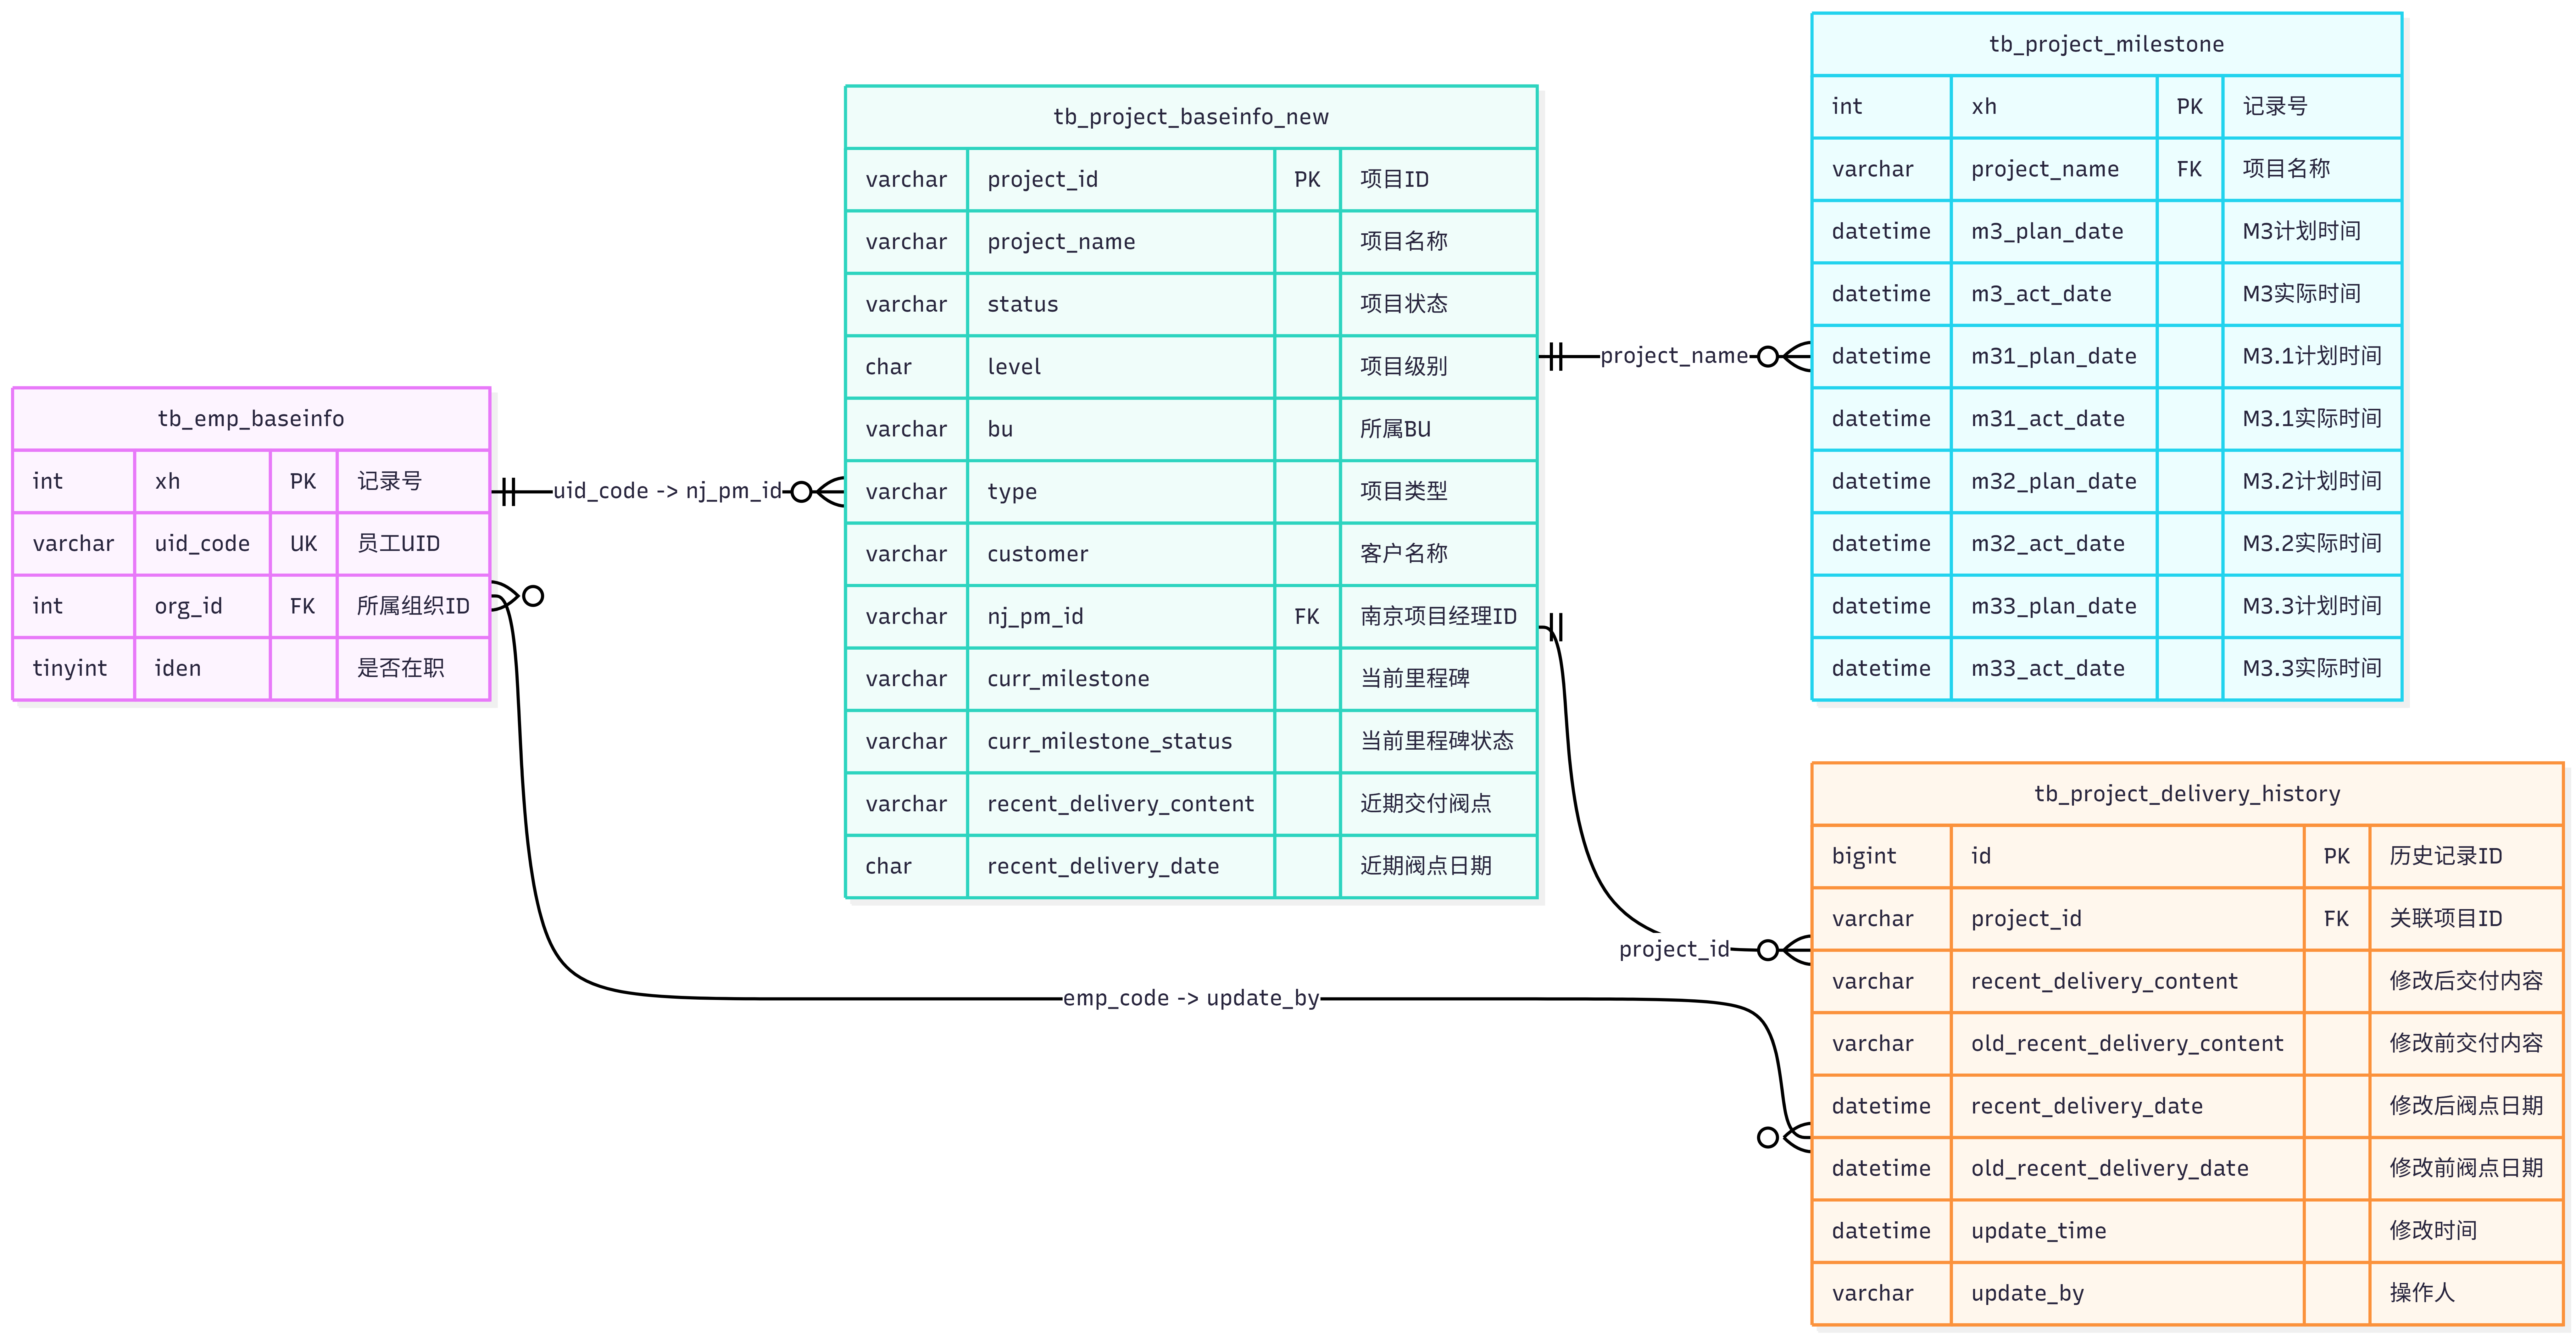
\includegraphics[width=0.7\linewidth]{imgs/ER图-项目代码.png}
		\caption{项目基本信息E-R图}
		\label{fig:er-project}
	\end{figure}
	
	项目基础信息表 \verb|tb_project_baseinfo_new| 是该模型中的核心实体，用于保存项目编号、项目名称、项目状态、项目级别、所属 BU、项目类型、客户名称、南京项目经理、当前里程碑和近期交付阀点等信息。员工基础信息表 \verb|tb_emp_baseinfo| 通过 \verb|uid_code| 与项目表中的 \verb|nj_pm_id| 建立逻辑关联，用于描述项目与南京项目经理之间的责任关系。
	\verb|tb_project_delivery_history| 用于保存项目近期交付内容的修改历史。当项目周报中的近期交付内容或交付日期发生变化时，系统会将修改前后的内容、修改时间以及操作人记录到该表中，从而实现项目交付信息的历史追溯。该表通过 \verb|project_id| 与项目基础信息表关联。\verb|tb_project_milestone| 用于记录项目 M3、M3.1、M3.2、M3.3 等关键阶段的计划时间和实际时间，通过 \verb|project_name| 与项目基础信息表形成逻辑关联。
	通过该 E-R 模型，系统能够支持项目基础信息分页查询、组合筛选、项目信息维护、里程碑维护和周报交付历史追踪等功能。
	
	
	\item 缺陷查询与统计模块需要整合来自 Trinity、Jira 和 BugClose 等多个缺陷平台的数据，并在此基础上支持项目维度和项目聚类维度的缺陷统计分析。其关系如图\ref{fig:er-bug-cluster}所示。
	
	\begin{figure}[htbp]
		\centering
		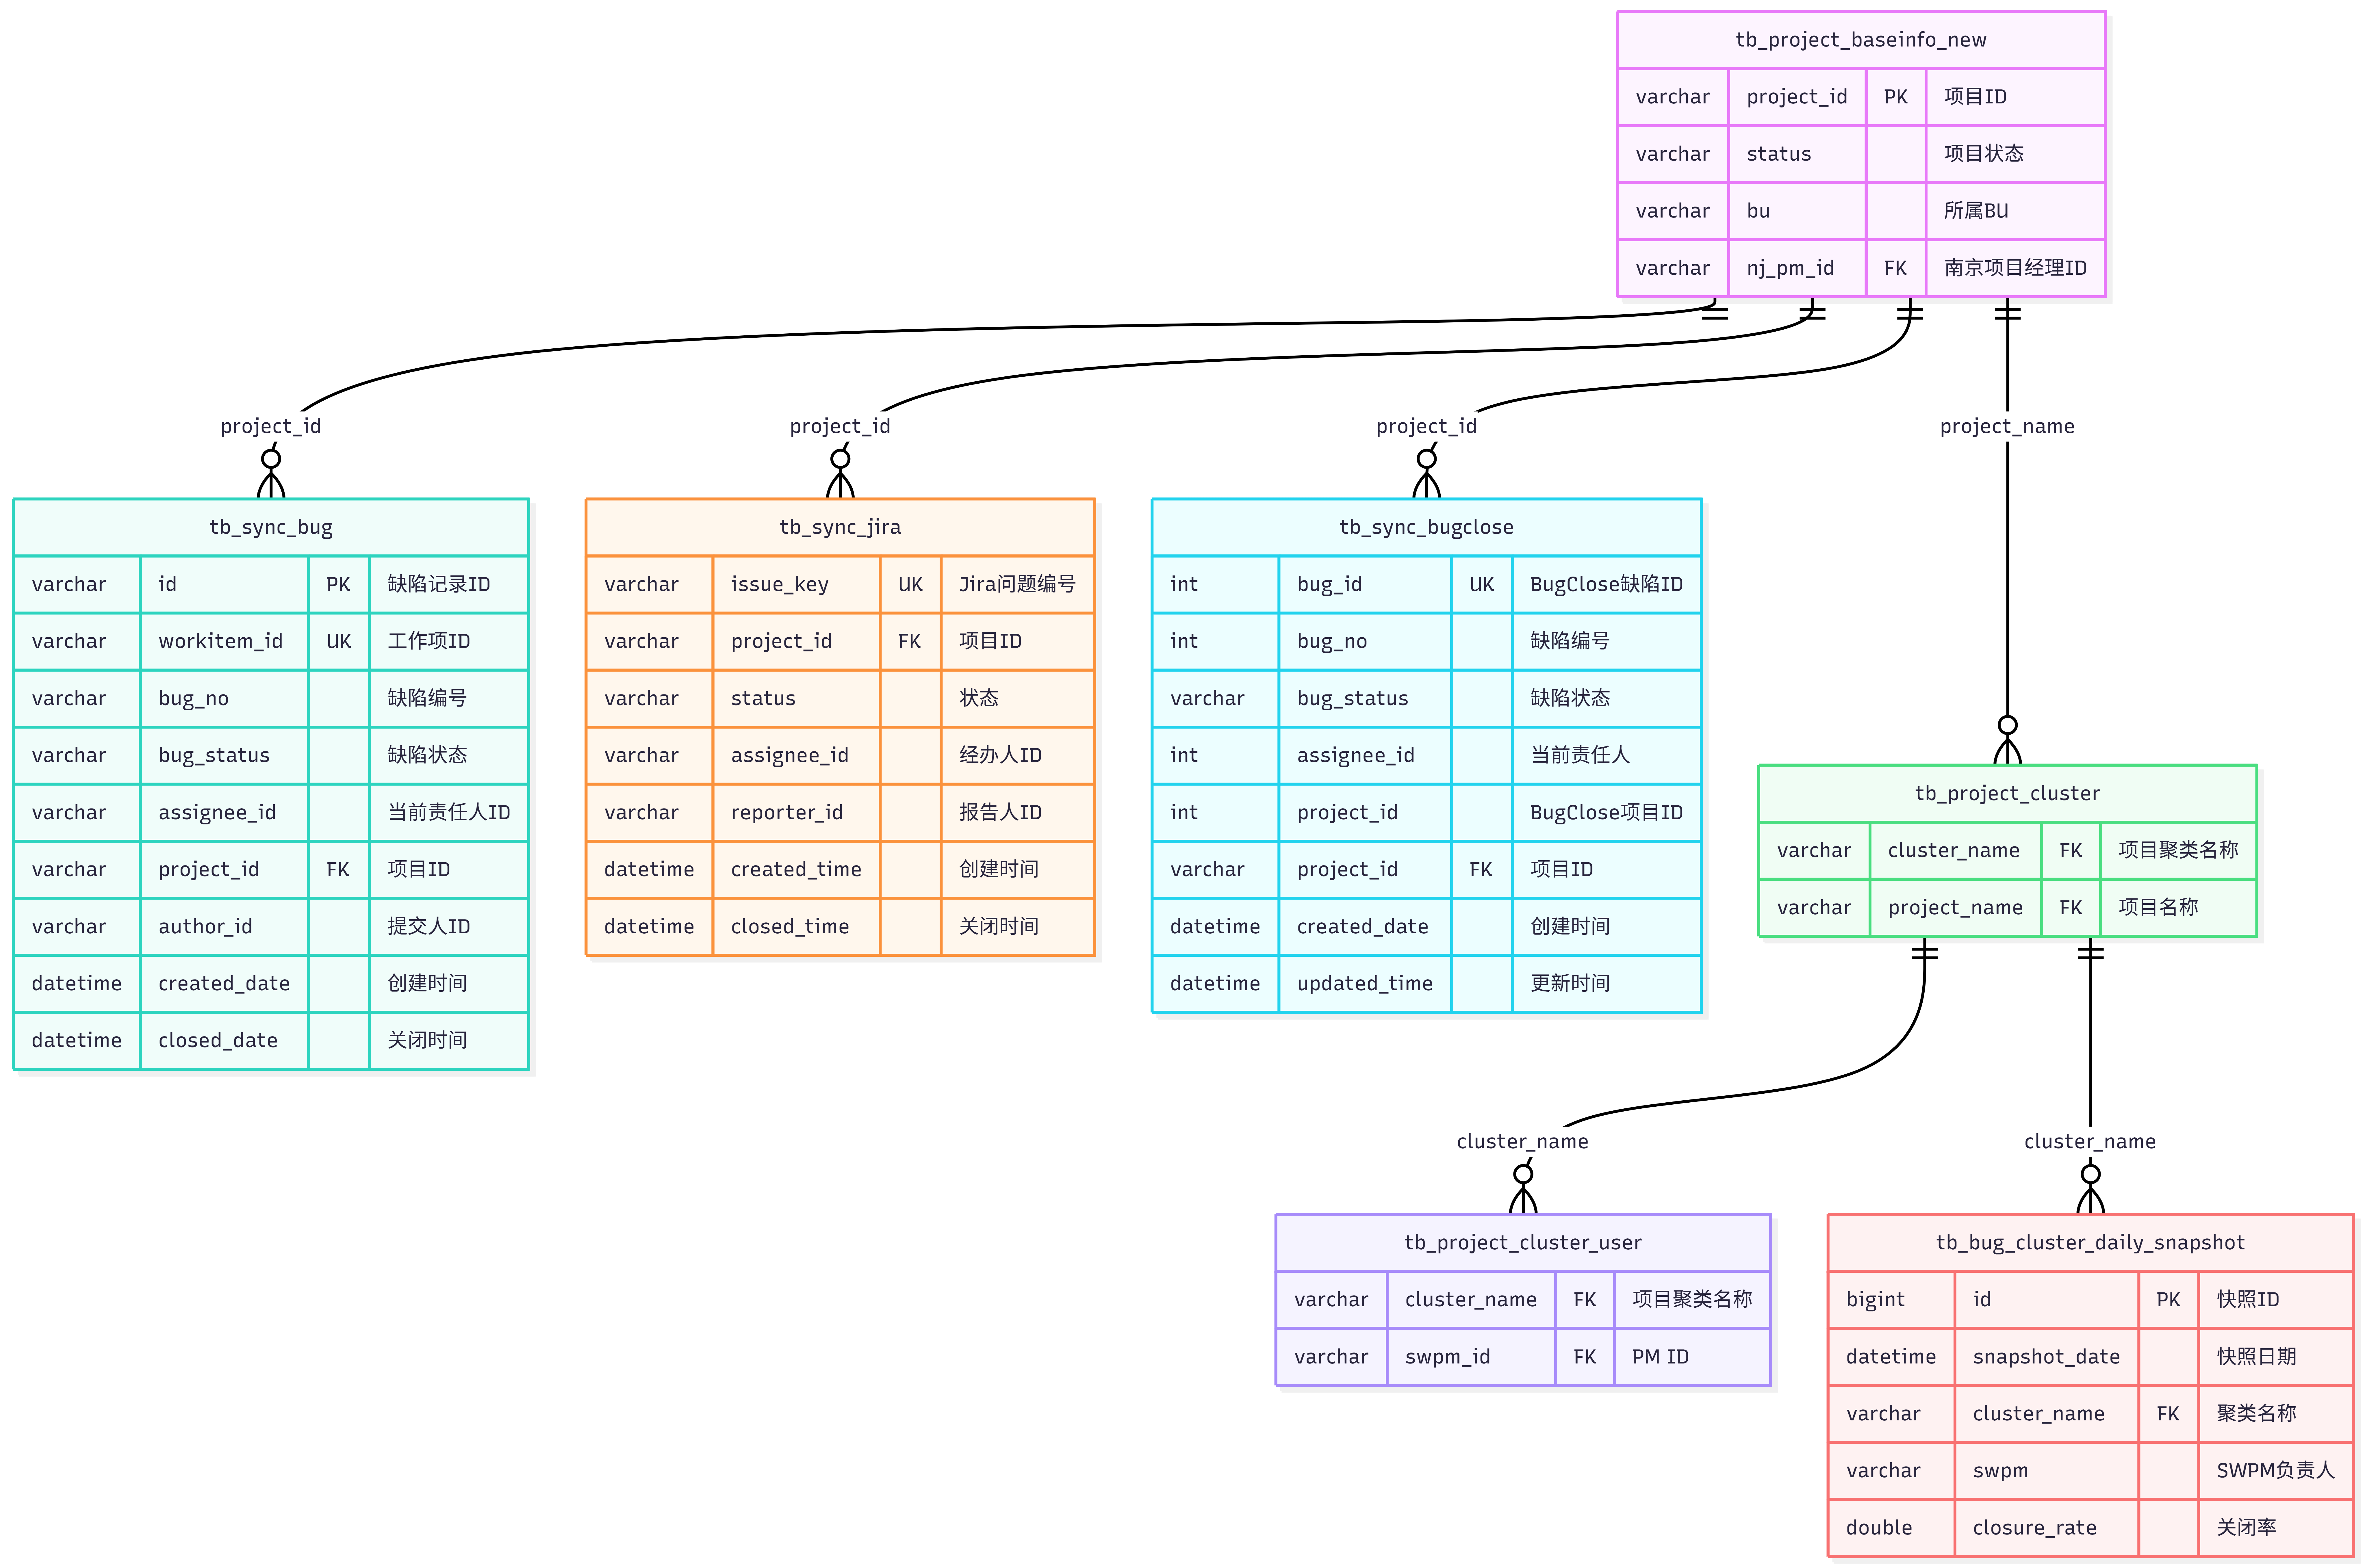
\includegraphics[width=0.7\linewidth]{imgs/ER图-缺陷聚类.png}
		\caption{缺陷聚类E-R图}
		\label{fig:er-bug-cluster}
	\end{figure}
	
	在该模型中，\verb|tb_project_baseinfo_new| 仍然作为项目主数据表，用于提供项目编号、项目状态、所属 BU 和项目负责人等基础信息。\verb|tb_sync_bug| 用于保存从 Trinity 系统同步的缺陷数据，包括缺陷记录 ID、工作项 ID、缺陷编号、缺陷状态、责任人、所属项目、创建时间和关闭时间等字段。\verb|tb_sync_jira| 用于保存从 Jira 系统同步的问题数据，包括 Jira 问题编号、问题状态、经办人、报告人、创建时间和关闭时间等信息。\verb|tb_sync_bugclose| 用于保存从 BugClose 系统同步的缺陷数据，包括 BugClose 缺陷 ID、缺陷编号、缺陷状态、责任人、所属项目和更新时间等字段。三类缺陷表均通过项目编号或项目名称与项目基础信息表建立逻辑关联。
	
	此外，系统使用 \verb|tb_project_cluster| 表维护项目与项目聚类之间的对应关系，使用 \verb|tb_project_cluster_user| 表维护项目聚类与 SWPM 负责人之间的对应关系，使用 \verb|tb_bug_cluster_daily_snapshot| 表保存项目聚类每日缺陷快照。通过这些表，系统可以按项目群或项目聚类维度统计未关闭缺陷数量、新增缺陷数量、关闭缺陷数量和关闭率等指标。该设计能够满足管理人员从单项目维度和项目群维度分析质量风险的需求。
	
	\item 重大问题管理模块用于记录项目研发和交付过程中出现的关键质量问题、交付风险和客户关注问题，其 E-R 模型如图\ref{fig:er-serious-problem}所示。
	
	\begin{figure}[htbp]
		\centering
		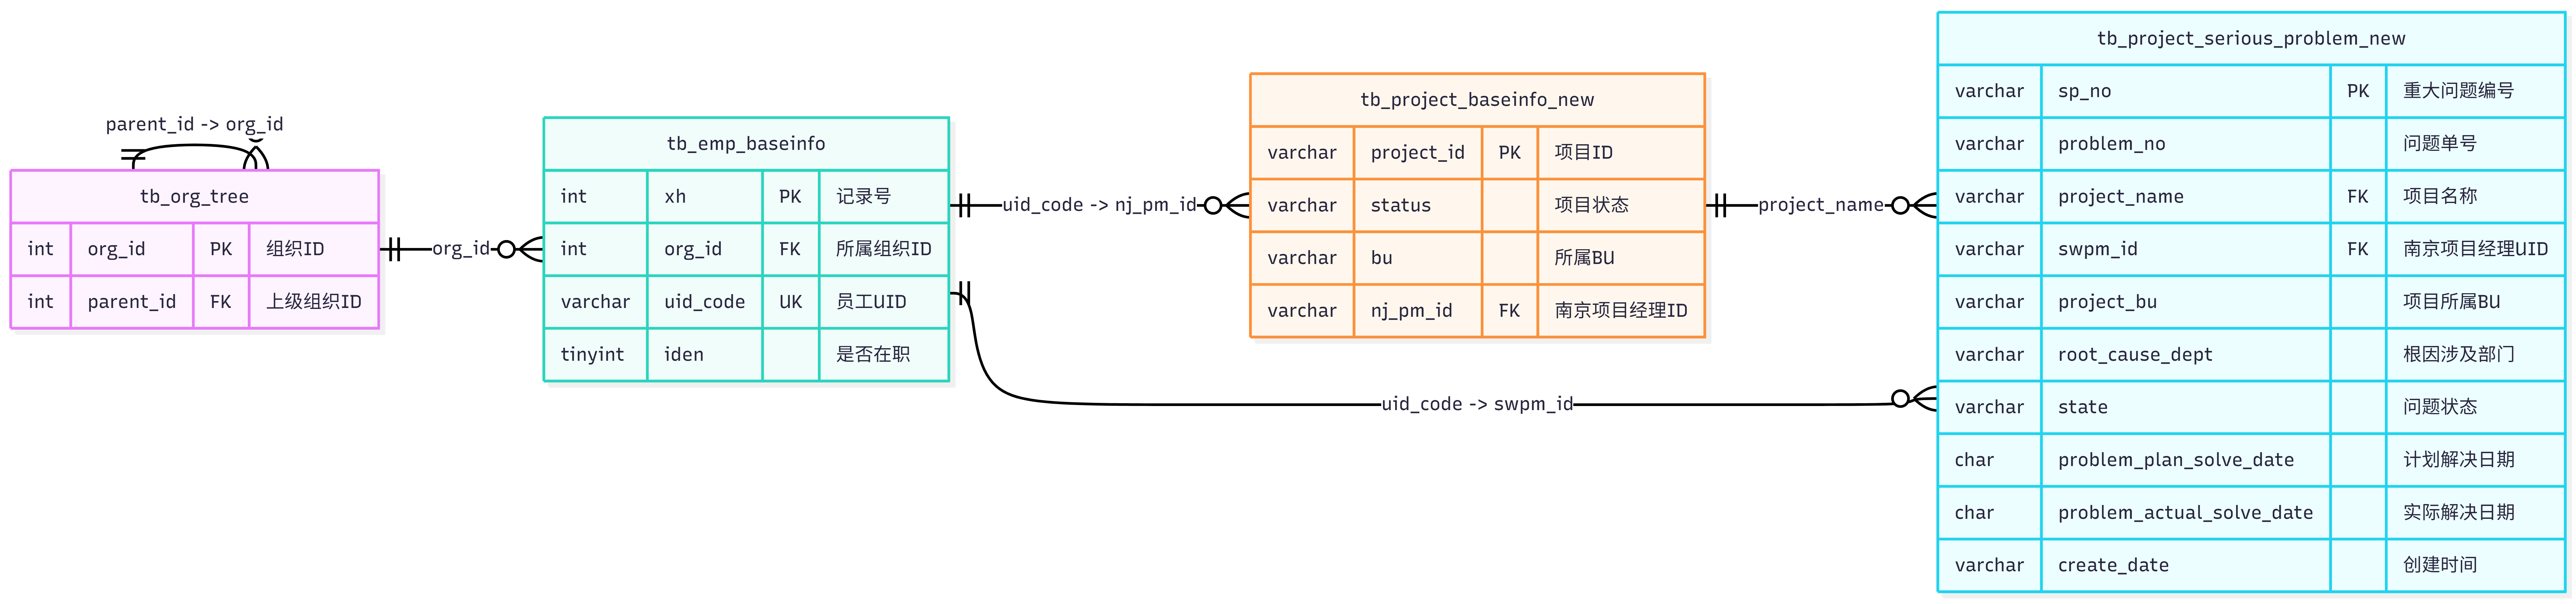
\includegraphics[width=0.7\linewidth]{imgs/ER图-重大问题.png}
		\caption{重大问题E-R图}
		\label{fig:er-serious-problem}
	\end{figure}
	
	该模型中，\verb|tb_project_serious_problem_new| 是重大问题管理的核心实体，用于保存重大问题编号、问题单号、项目名称、南京项目经理 UID、项目所属 BU、根因涉及部门、问题状态、计划解决日期、实际解决日期和创建时间等信息。项目基础信息表 \verb|tb_project_baseinfo_new| 通过项目名称与重大问题表建立逻辑关联，用于说明重大问题所属项目。员工基础信息表 \verb|tb_emp_baseinfo| 通过 \verb|uid_code| 与重大问题表中的 \verb|swpm_id| 建立逻辑关联，用于标识重大问题对应的南京项目经理。员工表又通过 \verb|org_id| 与组织表 \verb|tb_org_tree| 关联，从而可以进一步追溯问题涉及人员所属组织。
	
	通过该 E-R 模型，系统能够支持重大问题分页查询、新增、编辑、详情查看、状态跟踪和数据导出等功能。重大问题表不仅记录问题本身，还记录问题所属项目、责任人、根因部门和计划解决时间等关键管理信息，因此能够为项目复盘、质量改进和管理层决策提供数据依据。
	
\end{enumerate}
整体来看，四组E-R图分别从工时、项目、缺陷和重大问题四个维度，把系统的核心数据实体及其关联关系固定下来。建模过程遵循数据库设计总体原则。后续各功能模块的详细设计，均围绕本节E-R模型展开。

\section{本章小结}
本章重点论述了系统核心业务模块的详细设计，介绍了各个功能模块有关的类和接口以及关联关系，同时详细展示了几个关键点的具体设计和优化，给出了数据库中相关表结构的设计。下一章节，将基于系统的详细设计方案，展开对系统实现与测试的介绍。
\chapter{系统测试}

\section{测试环境与策略说明}

绪论部分主要论述选题的意义、国内外研	究现状以及本文主要研究的内容、研究思路以及内容安排等。

章标题为三号黑体加粗居中；一级节标题（如，2.1 本文研究内容）：四号黑体居左；二级节标题
（如，2.1.1 实验方法）：小四号宋体居左。

正文部分为小四号宋体，行间距 1.5 倍行距，首行缩进 2 个字符。正文一般不少于 15000 字。

\section{核心功能性测试}

\subsection{BU工时统计分析测试}

\subsection{项目基本信息管理测试}

\subsection{缺陷管理测试}

\subsection{重大问题管理测试}

相关模板和排版规则的整理可参见文献\cite{baker1995,desmarais1992}。……

\section{非功能性测试}

\subsection{缺陷查询深分页性能测试}

\subsection{工时统计界面优化}

\subsection{BU工时统计分析测试}

……

\chapter{总结与展望}

\section{工作总结}

本文所实现的数字化运营平台已经在公司内部使用，主要面向汽车电子软件项目管理和公司运营管理场景。本文围绕该平台的部分功能模块，完成了需求分析、系统设计、编码实现和功能测试等工作。

本文第一章分析了数字化运营平台的开发背景和国内外研究现状，介绍了论文的组织结构。第二章对系统用到的Spring Boot、Vue、MySQL、Redis、ECharts等关键技术做了简要说明。第三章从部门经理、项目经理、项目成员和质量人员四个角色，对BU工时统计分析、项目基本信息管理、缺陷管理和重大问题管理四个模块进行了功能性需求分析，同时从性能、可靠性和易用性等方面梳理了非功能性需求。第四章描述了 B/S 系统的五层架构，将整个平台按业务维度划分为系统管理、公司运营管理和项目运营管理三大模块，并说明了本文负责的后两个模块中各功能点的职责。第五章对四个模块的详细设计做了阐述，包括类图、时序图和数据库E-R模型。第六章展示了各模块的实现效果，通过功能测试用例和非功能性测试对系统进行了验证，其中针对缺陷深分页查询采用了延迟关联方案，优化后查询时间稳定在百毫秒级。

本次毕业设计具体负责的工作有：公司运营管理模块下的BU工时统计分析，支持按组织和年月维度查询各部门在业务单元上的工时投入，通过饼图和趋势图展示工时占比与变化趋势，利用Redis缓存减少数据库查询压力；项目运营管理模块下的项目基本信息维护，实现了项目的增删改查、条件筛选、Excel导出和交付历史追溯，采用主表加历史表的双写方式保留修改记录；缺陷管理模块，对接了Trinity、Jira和BugClose三个外部平台，采用策略模式与模板方法模式对多数据源查询接口进行重构，实现缺陷数据的统一查询和健康度分析；重大问题管理模块，实现了问题的新增、编辑、状态自动判定、飞书卡片通知和统计分析功能。

\section{工作展望}
本文设计实现的数字化运营平台已基本满足企业项目管理的日常需求，但在实际应用过程中仍暴露出一些不足之处，有待进一步优化和完善。未来的改进方向主要包括以下几个方面：
\begin{enumerate}[label=(\arabic*)]
	\item
	当前系统基于Spring Boot 2.1和Vue2构建，框架版本比较老旧，部分核心依赖已停止维护更新，存在潜在的安全风险。后续可以将前后端框架升级至Spring Boot 3.x，以便于引入 Spring AI 来让系统集成大模型服务，在缺陷分析、风险评估和项目报告生成等场景中探索智能化辅助能力。并迁移至 Java21 长期支持版本，因为这个版本的JDK提出了虚拟线程，非常适用于Web应用程序这种I/O密集型场景，前端每次启动速度都比较慢，可以考虑迁移至 Vue 3 配合 Vite 构建工具，以获得更好的性能和更完善的生态支持。
	
	\item
	目前平台已具备公司运营管理和项目运营管理两大功能域，能够为企业提供基本的数字化支撑。但从企业整体运营管理的视角来看，尚未覆盖企业运营管理的全部层级，后续可以在这个平台上继续扩展部门运营管理子系统，对部门级的人力资源效能、项目承接能力和团队协同效率做更细化的分析；同时可以考虑开发运营管理子系统，把需求吞吐量、代码提交频率、构建成功率等研发过程指标纳入平台，帮助团队发现开发流程中的瓶颈；还可以朝战略运营管理方向拓展，将各业务域的数据做更高层次的汇总，为管理层提供经营决策方面的数据支持。
\end{enumerate}

% 参考文献——看情况
\seuprintbibliography

\appendix
% 附录章节
% \input{content/appendix-a.tex}
% 致谢——注释
\chapter*{致\hspace{2em}谢}
\addcontentsline{toc}{chapter}{致\hspace{2em}谢}
转眼间，大学阶段的学习生活已接近尾声。回望这几年的求学经历，从最初面对专业知识时的陌生，到逐渐能够独立完成系统设计与实现，其中既有不断尝试后的收获，也有遇到困难时的迷茫与坚持。毕业论文的完成，不仅是对所学知识的一次总结，也是对自己学习能力和实践能力的一次检验。一路走来，许多人给予了我帮助和支持，在此谨向他们表达诚挚的感谢。

首先，衷心感谢我的指导老师廖力。在论文选题、系统设计、论文撰写和修改过程中，廖老师都给予了我耐心的指导和宝贵的建议。老师严谨的治学态度和认真负责的工作作风，使我在完成毕业设计的过程中受益良多。

其次，感谢我的父母一直以来的理解、支持和鼓励。他们在生活和精神上给予了我坚实的依靠，让我能够安心完成学业。也感谢姐姐在学习和生活中对我的关心与帮助，在我遇到压力和困难时给予鼓励和陪伴。

最后，也想感谢那个始终没有放弃的自己。无论是面对十字路口时的迷茫，还是付出努力却短时间内看不到结果，这一路走来都曾遇到过不少困难和压力。好在自己还是一步一步坚持了下来。

毕业不是终点，而是新的开始。今后我也会带着这段经历中的收获，继续踏实地走好接下来的路。
% 论文最后一页——注释
\seumottopage

\end{document}
